% CREATED BY DAVID FRISK, 2018

% IMPORT SETTINGS
\documentclass[12pt,a4paper,oneside]{report}
% CREATED BY DAVID FRISK, 2018

% BASIC SETTINGS
\usepackage{moreverb}								% List settings
\usepackage{textcomp}								% Fonts, symbols etc.
\usepackage{lmodern}								% Latin modern font
\usepackage{helvet}									% Enables font switching
\usepackage[T1]{fontenc}							% Output settings
\usepackage[english]{babel}							% Language settings
\usepackage[utf8]{inputenc}							% Input settings
\usepackage{amsmath}								% Mathematical expressions (American mathematical society)
\usepackage{amssymb}								% Mathematical symbols (American mathematical society)
\usepackage{graphicx}								% Figures
\usepackage{color, colortbl}
\usepackage{subfig}									% Enables subfigures
\numberwithin{equation}{chapter}					% Numbering order for equations
\numberwithin{figure}{chapter}						% Numbering order for figures
\numberwithin{table}{chapter}						% Numbering order for tables
\usepackage{listings}								% Enables source code listings
\usepackage{chemfig}								% Chemical structures
\usepackage{dirtytalk}                              % quotes
\usepackage[top=3cm, bottom=3cm,
			inner=3cm, outer=3cm]{geometry}			% Page margin lengths			
\usepackage{eso-pic}								% Create cover page background
\newcommand{\backgroundpic}[3]{
	\put(#1,#2){
	\parbox[b][\paperheight]{\paperwidth}{
	\centering
	\includegraphics[width=\paperwidth,height=\paperheight,keepaspectratio]{#3}}}}
\usepackage{float} 									% Enables object position enforcement using [H]
\usepackage{parskip}								% Enables vertical spaces correctly 



% OPTIONAL SETTINGS (DELETE OR COMMENT TO SUPRESS)

% Disable automatic indentation (equal to using \noindent)
\setlength{\parindent}{0cm}                         


% Caption settings (aligned left with bold name)
\usepackage[labelfont=bf, textfont=normal,
			justification=justified,
			singlelinecheck=false]{caption} 		

		  	
% Activate clickable links in table of contents  	
\usepackage{hyperref}								
\hypersetup{colorlinks, citecolor=black,
   		 	filecolor=black, linkcolor=black,
    		urlcolor=black}


% Define the number of section levels to be included in the t.o.c. and numbered	(3 is default)	
\setcounter{tocdepth}{5}							
\setcounter{secnumdepth}{5}	


% Chapter title settings
\usepackage{titlesec}		
\titleformat{\chapter}[display]
  {\Huge\bfseries\filcenter}
  {{\fontsize{50pt}{1em}\vspace{-4.2ex}\selectfont \textnormal{\thechapter}}}{1ex}{}[]


% Header and footer settings (Select TWOSIDE or ONESIDE layout below)
\usepackage{fancyhdr}								
\pagestyle{fancy}  
\renewcommand{\chaptermark}[1]{\markboth{\thechapter.\space#1}{}} 


% Select one-sided (1) or two-sided (2) page numbering
\def\layout{2}	% Choose 1 for one-sided or 2 for two-sided layout
% Conditional expression based on the layout choice
\ifnum\layout=1	% Two-sided
    \fancyhf{}			 						
	\fancyhead[LE,RO]{\nouppercase{ \leftmark}}
	\fancyfoot[LE,RO]{\thepage}
	\fancypagestyle{plain}{			% Redefine the plain page style
	\fancyhf{}
	\renewcommand{\headrulewidth}{0pt} 		
	\fancyfoot[LE,RO]{\thepage}}	
\else			% One-sided  	
  	\fancyhf{}					
	\fancyhead[C]{\nouppercase{ \leftmark}}
	\fancyfoot[C]{\thepage}
\fi


% Enable To-do notes
\usepackage[textsize=tiny]{todonotes}   % Include the option "disable" to hide all notes
\setlength{\marginparwidth}{2.5cm} 


% Supress warning from Texmaker about headheight
\setlength{\headheight}{15pt}		


% Tag command (invisible)
\newcommand{\tagtemp}{\textcolor{white}{, template by David Frisk}}

% Source code listings with Java syntax
% https://en.wikibooks.org/wiki/LaTeX/Source_Code_Listings
\lstset{
    language=Java,
    breaklines,
    deletekeywords={category},
    basicstyle=\ttfamily\footnotesize,
    otherkeywords={!,!=,~,\$,*,\&,\%/\%,\%*\%,\%\%,<-,<<-},
    literate={~}{$\sim$}1 {<-}{{$\gets$}}1
}

% Tables with colors
\definecolor{RowColor}{gray}{0.9}

\newcommand{\oneLineTitle}{SecArchUnit}
\newcommand{\multiLineTitle}[1]{SecArchUnit}
% The term [#1] indicates that there will be 1 rowbreak to split the title into two pieces, first part before \\[#1] and second part after. If you have a very long title and need to split it up into 3 rows, just use \\[#1] multiple times.

\newcommand{\oneLineSubtitle}{Extending ArchUnit to support validation of security architectural constraints}


\begin{document} 

% COVER PAGE, TITLE PAGE AND IMPRINT PAGE
\pagenumbering{roman}			% Roman numbering (starting with i (one)) until first main chapter
% CREATED BY DAVID FRISK, 2018

% COVER PAGE
\begin{titlepage}
\newgeometry{top=3cm, bottom=3cm,
			left=2.25 cm, right=2.25cm}	% Temporarily change margins		
			
% Cover page background 
\AddToShipoutPicture*{\backgroundpic{-4}{56.7}{figure/auxiliary/frontpage_eng.pdf}}
\addtolength{\voffset}{2cm}

% Cover picture (replace with your own or delete)		
%\begin{figure}[H]
%\centering
%\vspace{2cm}	% Adjust vertical spacing here
%
\includegraphics[width=0.9\linewidth]{figure/auxiliary/13067542-disguised-computer-hacker.jpg}
%\end{figure}

% Cover text
\mbox{}
\vfill
\renewcommand{\familydefault}{\sfdefault} \normalfont % Set cover page font
\textbf{{\Huge 	SecArchUnit: Extending ArchUnit to
support validation of security architectural constraints}} 	\\[0.5cm]
%{\Large A Subtitle that can be Very Much Longer if Necessary}\\[0.5cm]
Master's Thesis in Software Engineering \setlength{\parskip}{1cm}

{\Large MARCUS RANDEVIK \\[0.2cm]
        PATRIK OLSON} \setlength{\parskip}{2.9cm}

Department of Computer Science and Engineering \\
\textsc{Chalmers University of Technology} \\
Gothenburg, Sweden \the\year

\renewcommand{\familydefault}{\rmdefault} \normalfont % Reset standard font
\end{titlepage}


% BACK OF COVER PAGE (BLANK PAGE)
\newpage
\restoregeometry
\thispagestyle{empty}
\mbox{}


% TITLE PAGE
\newpage
\thispagestyle{empty}
\begin{center}
	\textsc{\large Master's thesis \the\year:NN}\\[4cm]		% Report number given by department 
	\textbf{\Large SecArchUnit: Extending ArchUnit to support validation of security architectural constraints} \\[1cm]
	%{\large A Subtitle that can be Very Much Longer if Necessary}\\[1cm]
	{\large MARCUS RANDEVIK}\\
	{\large PATRIK OLSON}
	
	\vfill	
	% Logotype on titlepage	
	\begin{figure}[H]
	\centering
	% Remove the following line to remove the titlepage logotype
	
\includegraphics[width=0.2\pdfpagewidth]{figure/auxiliary/logo_eng.pdf} \\	
	\end{figure}	\vspace{5mm}	
	
	Department of Computer Science and Engineering \\
	\emph{Division of Software Engineering}\\
	%Name of research group (if applicable)\\
	\textsc{Chalmers University of Technology} \\
	Gothenburg, Sweden \the\year \\
\end{center}


% IMPRINT PAGE (BACK OF TITLE PAGE)
\newpage
\thispagestyle{plain}
\vspace*{4.5cm}
SecArchUnit: Extending ArchUnit to support validation of security architectural constraints\\
%A Subtitle that can be Very Much Longer if Necessary\\
MARCUS RANDEVIK\\
PATRIK OLSON \setlength{\parskip}{1cm}

\copyright ~ MARCUS RANDEVIK, PATRIK OLSON, \the\year. \setlength{\parskip}{1cm}

Supervisor: Riccardo Scandariato, Computer Science and Engineering\\
Examiner: Michel Chaudron, Computer Science and Engineering \setlength{\parskip}{1cm}

Master's Thesis \the\year:NN\\	% Report number given by department 
Department of Computer Science and Engineering\\
Division of Software Engineering\\
%Name of research group (if applicable)\\
Chalmers University of Technology\\
SE-412 96 Gothenburg\\
Telephone +46 31 772 1000 \setlength{\parskip}{0.5cm}

\vfill
% Caption for cover page figure if used, possibly with reference to further information in the report
%Cover: Wind visualization constructed in Matlab showing a surface of constant wind speed along with streamlines of the flow. \setlength{\parskip}{0.5cm}

Typeset in \LaTeX \tagtemp\\
Printed by Chalmers Reproservice\\
Gothenburg, Sweden \the\year



%\todototoc
%\listoftodos

% ABSTRACT
\newpage
% CREATED BY DAVID FRISK, 2018
\oneLineTitle\\
\oneLineSubtitle\\
MARCUS RANDEVIK\\
PATRIK OLSON\\
Department of Computer Science and Engineering\\
Chalmers University of Technology and University of Gothenburg\setlength{\parskip}{0.5cm}

\thispagestyle{plain}			% Supress header 
\setlength{\parskip}{0pt plus 1.0pt}
\section*{Abstract}
The architecture of a software system heavily influences the level of security achieved.  However, a perfectly designed architecture does not provide any security if the implementation does not conform to the constraints. Adhering to a defined architecture is easier said than done as the representation of its design often requires manual labor to validate the conformance of the implementation. Previous attempts at solving the issue of creating a representation that allows for automatic conformance checking has failed to gain adoption, perhaps due to the disparity between models and code. In this thesis, we present our investigation and extension of the ArchUnit library to support the validation of security architectural constraints. In contrast to previously proposed approaches, ArchUnit represents architectural constraints via rules that can be validated using conventional unit test runners.  We compare our extension of ArchUnit, called SecArchUnit, to both SonarQube and PMD to distinguish any difference in their ability to detect violations of constrains as well as their appropriateness of expressing architectural constraints. Our results show that SecArchUnit was able to detect a wider variety of constraints and provides an interface more suitable for defining constraints at the architectural level.

% KEYWORDS (MAXIMUM 10 WORDS)
\vfill
Keywords: Software Architecture, Architectural Conformance, Static Analysis, Security

\newpage				% Create empty back of side
\thispagestyle{empty}
\mbox{}

% ACKNOWLEDGEMENTS
\newpage
% CREATED BY DAVID FRISK, 2018
\thispagestyle{plain}			% Supress header
\section*{Acknowledgements}
Lorem ipsum dolor sit amet, consectetur adipisicing elit, sed do eiusmod tempor incididunt ut labore et dolore magna aliqua. Ut enim ad minim veniam, quis nostrud exercitation ullamco laboris nisi ut aliquip ex ea commodo consequat. Duis aute irure dolor in reprehenderit in voluptate velit esse cillum dolore eu fugiat nulla pariatur. Excepteur sint occaecat cupidatat non proident, sunt in culpa qui officia deserunt mollit anim id est laborum.

\vspace{1.5cm}
\hfill
Name Familyname, Gothenburg, Month Year

\newpage				% Create empty back of side
\thispagestyle{empty}
\mbox{}


% TABLE OF CONTENTS
\newpage
\tableofcontents

% OTHER FRONTMATTER
% List of figures (add to table of contents)
\clearpage
\addcontentsline{toc}{chapter}{\listfigurename} 
\listoffigures
% List of tables (add to table of contents)
\clearpage
\addcontentsline{toc}{chapter}{\listtablename}  
\listoftables

%\clearpage
%\addcontentsline{toc}{chapter}{List of Listings}
%\lstlistoflistings


% START OF MAIN DOCUMENT
\cleardoublepage
\setcounter{page}{1}
\pagenumbering{arabic}			% Arabic numbering starting from 1 (one)
\setlength{\parskip}{10pt plus 1pt}

% INTRODUCTION
\chapter{Introduction}
In the age of an ever more digitalized world, ensuring the security of software systems becomes an increasingly critical task. The increased importance of security is true in particular, as systems are being developed based on the principle of permanent connectivity \cite{felderer_security_2016}.  Services ranging from those offered by governmental agencies to that of social media are always connected to the open internet, potentially creating a large surface of attack. Although the importance of a securely designed system is widely known, developing a secure system is a challenging task. Far from all software engineers are security specialists, or for that matter, particularly educated in security aspects \cite{yoshioka_survey_2008}.

Introducing a weakness into a system can be done in every part of the software development lifecycle. An early introduction often leads to a more costly fix as the scope of the flaw is increased \cite{mcgraw_software_2004}. Typically, weaknesses are categorized as either implementation bugs (e.g. buffer overflow) or design flaws (e.g. client-side validation) where the later commonly has a more extensive scope and is the responsibility of the architect \cite{arce_avoiding_2014}. However, this binary division might be too simplified as it assumes a secure design is implemented correctly, meaning that there is no discrepancy between the "intended architecture" and the actual one found in the source code. Jasser \cite{franch_constraining_2019} considers violations of the architectural security design as a third type of category with a comparable impact to that of design flaws.

Deviations from the intended architecture are not unique to the initial implementation of a system. Over time, subsequent changes made to the system, often due to new requirements, frequently lead to further disparency called software erosion \cite{de_silva_controlling_2012}. Proponents of the agile methodology also somewhat worsen the problem of erosion as the reduction of upfront design severely hinders the design of the architecture \cite{van_gurp_design_2002}. Many of the tools and techniques produced by academia to try and remedy the frequent violations of architectural design have failed to gain wide adoption in the industry \cite{de_silva_controlling_2012}.  Of the few that have, architectural design documentation is the most prominent and widely included in numerous software processes. While the technique is well adopted, performing it formally to allow for automatic conformance monitoring is seldom done, causing developers to rely on the less scalable method of manual reviews \cite{de_silva_controlling_2012}.

A recently developed tool called ArchUnit\footnote{\url{https://www.archunit.org/}} has provided architects with the capability of validating architectural constraints using Java unit testing frameworks. While ArchUnit is not the first tool developed for architectural conformance checking, it is possibly the first to leverage already existing testing infrastructure (unit testing) in a manner that allows for testing over time. In its current form, ArchUnit has not provided any explicit functionality to test security constraints. Thus, the objective of this thesis is to explore the feasibility of expressing and enforcing typical security architectural constraints trough ArchUnit.

\section{Research questions}
To fulfill the objective of the study, the following research questions have been defined:

\begin{itemize}
    \item RQ1: What architectural security constraints can be validated using ArchUnit?
    \item RQ2: What modifications can be made to ArchUnit in order to facilitate the validation of additional constraints?
\end{itemize}

These questions are answered by first gathering a set of constraints from previous literature in the domain of architectural security. Secondly, we map the constraints to functionality already provided by ArchUnit and identify areas of extension. Lastly, we apply the constraints to a set of open-source systems to experimentally determine how reliably the tool detects violations of said constraints. Additionally, we compare ArchUnit to two static analysis tools to determine whether ArchUnit provides any improvements over existing tools. 

\section{Research contribution}
This work shows how architectural security constraints can be validated with the help of a static analysis tool. The thesis demonstrates the application of the tool to several open source system, in an evaluation of its precision and efficacy in terms of validating the constraints, and compares this to existing tools. In addition, a qualitative comparison is made between ArchUnit and existing tools in terms of their appropriateness for validating architectural security constraints.

\section{Limitations}
\label{sec:limitations}

This thesis, and the modified version of ArchUnit, is not intended to be a complete solution for all security architectural constraints. Instead, the study is performed to provide an initial evaluation of the possibility of using ArchUnit as an alternative to existing techniques of static conformance checking. 

The constraints that are considered in our work could be enforced through static analysis of Java bytecode. Any measure related to the configuration (of an application or operating system), the file-system, or other run-time properties that cannot be validated through static code analysis was deemed to be out of scope. 

Although the principle of ArchUnit may very well apply to programming languages other than Java, the limited scope of the thesis makes it unfeasible to provide functionality to analyze source-code in additional languages.

\section{Thesis outline}

The remainder of this report is structured as follows.

Chapter 2: Provides a general background to the topic of software architecture and architectural security constraints. In addition, the ArchUnit library is introduced and compared to previously developed tools for architectural conformance.  

Chapter 3: Presents our methodology of identifying a set of statically enforceable constraints as well as the experimental setup. 

Chapter 4: Contains the complete list of identified constraints and the final list of constraints selected for the evaluation with a detailed description of each. 

Chapter 5: Showcases how the constraints are expressed within ArchUnit and the identified gaps in functionality.

Chapter 6: Presents the results of our evaluation, a discussion of the inferences and answers to the research questions. 

Chapter 7: Concludes our work and outlines examples of future research.

% THEORY
\chapter{Background}

This chapter provides background knowledge regarding software architecture and architectural security constraints. The ArchUnit library is introduced and related to tools and approaches used in previous research.

\section{Software architecture}
The intention of this study is not to contribute to the definition of software architecture, though, our work relies on a shared understanding of what constitutes as the architecture of a system. This section presents the concept of software architecture and the definitions considered in our study.   

During the 1970s,  the idea of organizing software into distinguishable structures was initially introduced. Djikstra \cite{dijkstra_structure_1968} organized the system into a hierarchy of layers, each being dependent upon the interface of the layer below. Parnas discussed the criteria used to modularize systems \cite{broy_criteria_1972}, i.e. responsibility assignment, which allowed for independent development. Further, he introduced the concept of program families \cite{parnas_design_1976} where a set of systems share much of their functionality, allowing for a common design. The work on product families was later extended to describe the process of designing systems that support extensions by using abstracted components \cite{parnas_designing_1979}. 

However, the term \textit{software architecture} was formally introduced by Perry and Wolf in \cite{perry_foundations_1992}, where they defined software architecture as:

\[ Software \;  Architecture = \{elements,form,rationale\} \]

In words, software architecture is defined as a set of architectural elements that persist in a particular form. Form relates to the properties of each element and the relationship between elements. To make an architecture explicit, Perry and Wolf \cite{perry_foundations_1992} suggest the usage of views to represent different aspects of the architecture. 

Related to that of a specific architecture, Perry and Wolf \cite{perry_foundations_1992} define an architectural style as a generalization of various similar architectures. Garlan and Shaw \cite{ambriola_introduction_1993} extended the knowledge by providing a list of architectural styles that were commonly used in the design of software systems, these include \textit{pipes and filters}, and \textit{layered systems}. Perhaps more importantly, Garlan and Shaw \cite{ambriola_introduction_1993} describe the rationale of using a specific style and the trade-offs between styles.

Today, there are mainly two definitions of software architecture:

\begin{itemize}
    \item \textbf{Bass et Al \cite{bass_software_2013}}: \say{The software architecture of a program or computing system is the structure or structures of the system, which comprise software elements, the externally visible properties of those elements, and the relationships among them.}
    \item \textbf{Jansen and Bosch \cite{jansen_software_2005}}: \say{The composition of a set of architectural design decisions} where a design decision represents \say{A description of the set of architectural additions, subtractions and modifications to the software architecture, the rationale, and the design rules, design constraints and additional requirements that (partially) realize one or more requirements on a given architecture.}
\end{itemize}

While both definitions acknowledge that a system should always meet the functional requirements and that the process of creating the architecture is a balance between quality attributes, it is the former definitions that lend itself naturally to structural analysis.

Finally, in many references to architecture, the term design is often used ambiguously. To remedy this, Eden and Kazman \cite{eden_architecture_2003} formalized the hypothesis of an intension and locality criteria. A specification is said to be intensional if there are infinitely many ways of realization, all others are extensional. Further, a specification is said to be local if it only affects a small part of a program. Architectural specifications are both intensional and non-local, whereas design level specifications are intensional and local.

\section{Architectural security constraints}

The purpose of software and architectural security is to ensure that no harm occurs to the systems assets in the presence of malicious actors \cite{mcgraw_software_2004}. Assets are identified by the needs of the systems stakeholders and may be tangible (e.g, cash) or intangible (e.g, information) \cite{haley_security_2008}. At the core of software security are the following four concerns, often refereed to as CIAA:

\begin{itemize}
    \item \textbf{Confidentiality}, \say{Preserving authorized restrictions on information access and disclosure.} \cite{ross_systems_2018}
    \item \textbf{Integrity}, \say{Guarding against improper information modification or destruction.} \cite{ross_systems_2018}
    \item \textbf{Availability}, \say{Ensuring timely and reliable access to and use of information.} \cite{ross_systems_2018}
    \item \textbf{Accountability}, \say{Ensuring that it is possible to trace security relevant actions (i.e., subject-object interactions) to the entity on whose behalf the action is being taken} \cite{ross_systems_2018}
\end{itemize}

These concerns relate to a system's security goals as a violation of a concern to one of the assets describes a possible threat \cite{haley_security_2008}. Security requirements later operationalize the security goals and constrain the architecture of a system. As security is often considered a quality attribute, the satisfaction of a security requirement becomes a risk management issue.  Highly valuable assets should warrant a higher degree of protection and consequently, require stronger constraints on the architecture \cite{broy_software_2007}.

While the term architectural constraint means refers specifications that impact the structures of a system, and the relationships between them, several concepts and techniques have come to form a generalizable knowledge of solutions, at different levels of abstraction, that serve as constraints to satisfy the requirements. The concepts outlined below have definitions that vary across authors; thus, our goal is not to provide conclusive definitions but rather an overview. 

\textbf{Security principles}, such as those proposed by OWASP\footnote{\url{https://blog.threatpress.com/security-design-principles-owasp/}}, are defined at a level of high abstraction that allows them to be used on almost any component in a system. Examples of such principles include \textit{The principle of least privilege}, stating that any user should have the least amount of privileges needed to perform an action. While the abstraction of principles enables them to apply to most components of a system, it also means that an architect has to assess, instead of precisely knowing, whether the constructed architecture conforms to the principle. 

\textbf{Architectural tactics}, introduced by Bass et al in \cite{bass_software_2003}, refers to \say{a design decision that influences the achievement of a quality attribute respone}. In particular, security tactics aim to control the security response of a system, i.e. ensuring that the security goals always hold true. The original list of security tactics has later been refined \cite{ryoo_revising_2012,fernandez_revisiting_2015} and includes techniques for detecting, resisting, reacting to and recovering from attacks, as seen in Figure~\ref{fig:security_tactics}. Much like principles, tactics lack a common realization causing the architect to subjectively asses whether the tactic is implemented.

\begin{figure}
    \centering
    \captionsetup{justification=centering}
    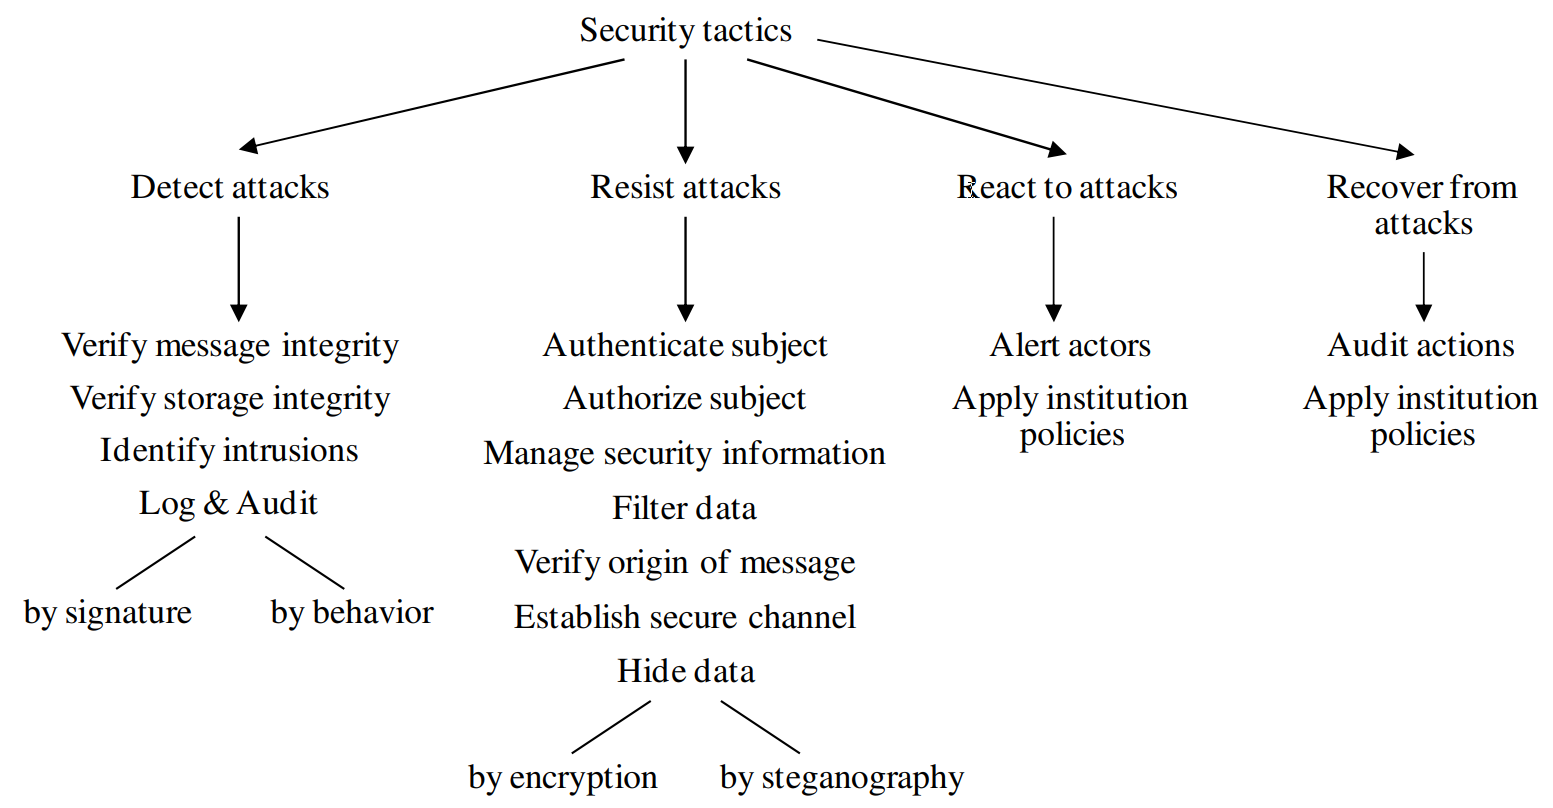
\includegraphics[width=\textwidth]{figure/securityTactics.png}
    \caption{A hierarchical tree of security tactics, adapted from \cite{fernandez_revisiting_2015}.}
    \label{fig:security_tactics}
\end{figure}

\textbf{Security patterns} are at a lower level of abstraction as they represent \say{encapsulated solutions to recurrent system problems} \cite{fernandez-buglioni_security_2013}. By composing a set of tactics in a generalizable solution to a known problem, patterns help to bridge the gap between the developers and the architectural experts \cite{rosado_study_2006}. The extensive knowledge of security patterns and their implementation also allows for comparisons in terms of their impact on other quality attributes, such as maintainability and performance \cite{scandariato_architecting_2009}. 

\textbf{Security rules}, while not as established in the literature, has come to serve as a less solution-oriented version of patterns. Rules often define dependencies, such as \say{Layer X must not access layer Y}, but may also define behavioral aspects. Much of the commonly used rules are tacit knowledge, meaning that there are few explicit mentionings. 

\section{ArchUnit}\label{archunit-back-section}
ArchUnit is a library that leverages static analysis to validate architectural constraints. Static analysis refers to the analysis of code, either in the shape of source code or compiled bytecode, without executing the code itself \cite[p. 21]{chess_secure_2007}. In the case of ArchUnit, the analysis is performed on compiled Java bytecode.

Using ArchUnit, the bytecode of a target system is analyzed and composed into a Java code structure \cite{gafert_archunit_2020}. This structure contains a number of classes, outlined in Figure~\ref{fig:archunit}, which describe the code of the analyzed system. As shown in the figure, ArchUnit introduces the following terminology:

\begin{figure}
    \centering
    \captionsetup{justification=centering}
    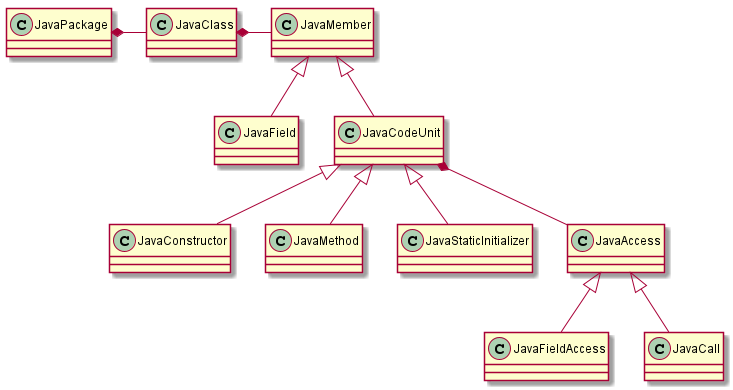
\includegraphics[width=\textwidth]{figure/ArchUnit.png}
    \caption{A UML class diagram of the code structure that ArchUnit uses to represent a system under analysis. Predicates and conditions are defined in terms of the classes in this structure. Figure adapted from \cite{gafert_archunit_2020}.}
    \label{fig:archunit}
\end{figure}

\begin{itemize}
    \item Methods, constructors and static initializers, i.e. anything that contains code statements, are collectively referred to as \textbf{code units}.
    \item Fields and code units, i.e. constructs that are owned by a class, are referred to as \textbf{members} of that class.
    \item Field accesses, method calls and constructor calls are collectively known as \textbf{accesses}. An access has a source, i.e. the code unit from which the access originates, and a target, i.e. the member that is being accessed.
\end{itemize}

The validation of a constraint is performed by evaluating one or multiple conditions against elements of this code structure. ArchUnit exposes a sentence-like API that allows these constraints to be expressed as sentences of the form \say{The \textbf{constructs} that match \textbf{predicate} should fulfill \textbf{condition}.} 

An example of a constraint can be seen in Listing~\ref{lst:architectural_rule}. This constraint assumes that there are two layers \textit{view} and \textit{controller}, in the form of packages, and dictates that the view layer should only be accessed by the controller layer. In this example, the constructs are classes (line 1), the predicate selects classes declared in a package with the suffix \textit{view} (line 2), and the conditition applied to these classes is that they should only be accessed by code units declared in a package with the suffix \textit{controller} (line 3).

\begin{center}
\begin{minipage}{0.90\linewidth}
\begin{lstlisting}[caption={Example of an architectural rule in ArchUnit.}, captionpos=b, label=lst:architectural_rule, numbers=left]
ArchRule rule = classes()
    .that().resideInAPackage("..view")
    .should().onlyBeAccessed().byAnyPackage("..controller");
\end{lstlisting}
\end{minipage}
\end{center}

In general, constructs refer to either classes, fields, methods or constructors. The predicate is used to filter the constructs based on their attributes, such as selecting classes that are defined in a specific package as seen in the example above. Finally, the condition is applied to all the selected constructs. Constructs that fail to fulfill the condition are reported as violating the constraint.


% \cite{pistoia_survey_2007}

% constraints can be enforced both statically and dynamically, as covered in related work
% ArchUnit employs static analysis; explain briefly what it means
% This, combined with constraints that can be validated with unit testing infrastructure, enables the tool to be used as part of a continuous integration pipeline
% These constraints are expressed in Java code and can be validated using conventional unit testing frameworks. 


\section{Related work}
This section presents existing approaches to architectural conformance monitoring and notations for expressing security concerns, and how they relate to this work.

\subsection{Architectural conformance monitoring}

In one approach to architectural conformance monitoring called ArchJava, presented by Aldrich et al. \cite{aldrich_archjava_2002}, the Java language is extended with syntax for describing architectural elements such as components and connectors. Constraints on these architectural elements are validated at compile-time, allowing violations to be caught at an early stage of development.

Abi-Antoun and Barnes \cite{abi-antoun_analyzing_2010} present a two-tiered approach to architectural conformance monitoring called SECORIA. Their approach utilizes code annotations and static analysis to extract an architectural representation of a system. This representation is then compared to a target architecture, which is modeled separately in an Architecture Description Language (ADL), in order to detect discrepancies between the intended architecture and the actual implementation.

De Silva \cite{de_silva_towards_2014} presents PANDArch, another two-tiered approach, in which the intended architecture is modeled using an ADL and checked for conformance with the actual implementation. As opposed to SECORIA, PANDArch utilizes dynamic analysis to extract the implemented architecture during executions of the system. 

The approach used by ArchUnit allows architectural constraints to be expressed directly in the source code, replacing the need for a separate model of the intended architecture. In addition, these constraints can be validated using existing unit test runners, enabling the tool to be used as part of a continuous integration pipeline.

%Comparison of static approaches
%\cite{knodel_comparison_2007}

%\cite{luckham_event-based_1995}
%\cite{de_silva_controlling_2012}



\subsection{Design annotations and security notations}

Sabo and Porubän \cite{sabo_preserving_2009} use Java annotations to preserve the correct form of design patterns during implementation. While the approach does not focus on security, the study showcases how constraints can be applied directly to the source code. Additionally, Sabo and Porubän argue that storing constraints at the location of its implementation increases developer awareness. 

Similarly, Sulir et al. \cite{sulir_recording_2016} record the developer's intentions (including security concerns) using source code annotations. They showed through two controlled experiments that annotations helped improve program comprehension and the correctness of the implementation.

Both SecureUML by Lodderstedt el al. \cite{goos_secureuml_2002} and UMLsec by Jürjens \cite{goos_umlsec_2002} propose extensions to UML to incorporate security-relevant information to allow for formal reasoning and evaluation. While SecureUML focuses solely on access control, specifically role-based access control, UMLsec provides more general constructs.

While SecureUML and UMLsec define concepts at a relatively low level of abstraction to allow for the generation of access control infrastructure for the former, and formal verification for the latter, Sion et al. \cite{sion_masc_2015} propose another set of extensions aimed at concerns on the architectural level. The extensions are based on two sets of security design concepts: (1) \say{well-known and often-used security concepts or techniques} and (2) \say{security goals and objectives}. As a consequence of the focus on architectural level concerns, much of their extension to UML are graphical elements rather than stereotypes and tagged values, as in the previous examples. 

A systematic review of the field by van den Berghe et al. \cite{vandenberghe_design_2017} revealed that of the many proposed notations for security, few had any existing tool support outside of a vaguely mentioned prototype. Additionally, the coverage across security concerns was not equal. Most notations covered aspects of access-control but lacked support for most of the CIAA concerns. 

Our approach tries to extend the field of security notation by applying them to architectural conformance testing. We utilize annotations, in the shared belief of \cite{sabo_preserving_2009} that constraints should be applied closest to their implementation. While the use of formal models allows for rigorous proofs, we believe a more lightweight model can be a complement in settings where formality becomes too large of an overhead, such as in agile environments. 

% METHODS
\chapter{Methodology}

This chapter describes the adopted method for collecting relevant constraints, relating these to the common security-goals of CIAA, and later mapping them to functionality within ArchUnit. Second, this chapter presents the validation plan for expressing security constraints with ArchUnit, both by comparing it to industry used static analysis tools and a separate analysis focusing on constraints that could only be expressed in ArchUnit.

\section{Identification of design constraints}

The evaluation of SecArchUnit was based on the reliability to detect violations of security architectural constraints. In the absence of any pre-existing set of constraints, the first part of our study was devoted to collecting relevant constraints. The following sections describe the two-part process of collecting and filtering said constraints. 

\subsection{Data collection} \label{sec:data_collection}

The relevance of the security architectural constraints included in the study was ensured by performing a review of security measures and common weaknesses and compiling the result to a list of constraints. Completeness was not the primary goal of the review, but rather to provide a set of constraints derived from previous knowledge. Presented below are the three sources used to form the final list. 

\textbf{CAWE catalog:}
The Common Architectural Weakness Enumeration catalog \cite{santos_catalog_2017} details 224 common weaknesses in security architectures. Each entry has a description of the weakness and exemplifications of how it could manifest itself in the source code, when applicable. In some entries, there are recommendations on what techniques can be used to detect the weakness, along with mitigation strategies.

\textbf{Security patterns:}
Similar to the usage of general design patterns made famous in \cite{gamma_design_1995}, security patterns provide a reusable and domain-independent solution to a known problem. More specifically, this study focused on security patterns for the design phase, as defined in \cite{yoshioka_survey_2008}. While the security pattern repository\footnote{\url{http://sefm.cs.utsa.edu/repository/}} lists over 170 security patterns, not all are provided with sufficient detail or at the appropriate level of abstraction. As a result, the report by Scandariato et al. \cite{scandariato_system_2006}  which provides a filtered list of patterns.


\textbf{Security rules:} \label{subsec:security_rules}
Architectural security rules constrain the implementation of a system while being less solution-oriented compared to security patterns. Eden and Kazman differentiate architectural security rules from those defined on a level of source code based on two criteria, locality and intension/extension \cite{eden_architecture_2003}. Architectural rules are both non-local and intensional, meaning that they affect all or several parts of the system while having \say{infinitely-many possible instances}. In \cite{franch_constraining_2019}, Jasser presents a catalog of architectural security rules. Although the entire catalog of 150 security rules is not yet available, the initial list of 22 included in the paper was used in our study.

\subsection{Filtering}\label{sec:processing}

%Elaborate. Perhaps explaining how the sources were analyzed. Did you analyse one right after the other, were there iterations, did you meet after each iteration to discuss your findings and synchronize individually derived subset, or did you work together? How many constraints were taken from individual sources, which of those were grouped? What is the proportion of CIAA coverage in the final list (Show CIAA in table 4.2 and show #ID linking the chosen ones from 4.1)? What was the rational for grouping? Perhaps explicitly enumerating  the "rules" you followed for inclusion would be nice (if there are more than two :) ...), e.g.:
%1) only security related architectural constraints were considered
%2) only constraints that can be enforced statically (FYI: prepare for the question, what is an example of a constraint that can not be statically enforced?),
%3) ...
Starting from each of the three sources of architectural constraints described in Section~\ref{sec:data_collection}, the first step of the process, shown in Figure~\ref{fig:mapping_process}, was to select the entries that could be formulated as enforceable constraint in the context of our project. The criteria for inclusion were the following: 

\begin{enumerate}
    \item The entry must be related to the architectural design of a system, i.e., non-local and intensional (as described in Section~\ref{subsec:security_rules}). \label{criterion_1}
    \item It must be possible to enforce the entry through static analysis. An example on a non enforceable constraint is \say{No two instances of a microservice are deployed on the same machine} \cite{franch_constraining_2019}, as the number of machines deployed is a dynamic property. \label{criterion_2}
    \item Although somewhat included in the first criterion as it is a local issue, an entry must not relate to the correctness or best practice of the implementation of an algorithm. Examples include the practice of using session tokens with time-limited validity. \label{criterion_3}
    \item The entry must only relate to the system under design, thus ignoring the correctness and security of any external dependencies. An example can be found in SonarQube where the usage of a version of a library with known vulnerabilities is reported as a weakness. \label{criterion_4}
    \item The entry must not be dependent on externally defined data. A common example is that of user permissions where the mapping between a regulated function and a users rights is performed using an access control list, external to the source code. \label{criterion_5}
    \item Additionally, we deemed entries defined as the absence of certain functionality as less valuable due to the increased difficulty of enforcing them \cite{haley_security_2008}. An example of such an entry is \say{The system must not provide functionality to decrypt secured log messages}, as defined in \cite{franch_constraining_2019}.
\end{enumerate}

\begin{figure}
    \centering
    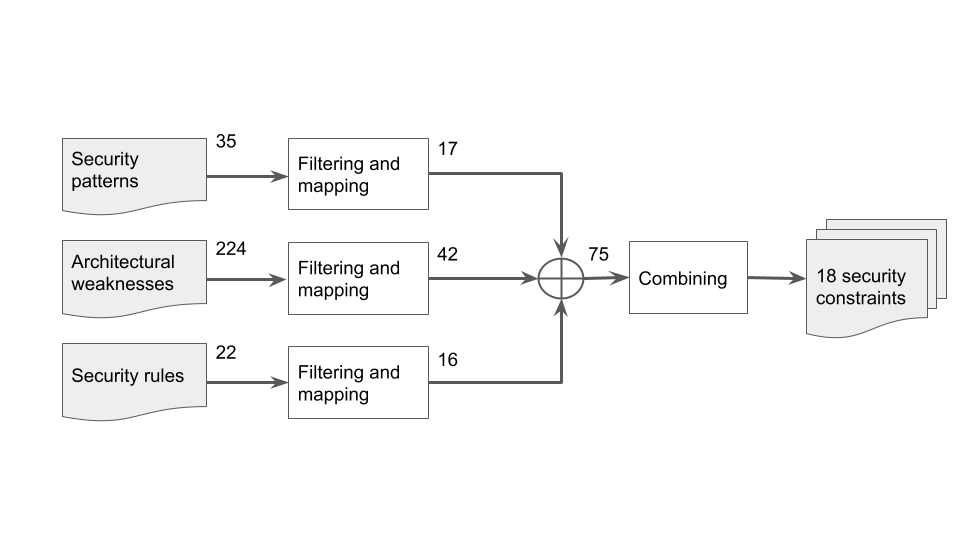
\includegraphics[width=\textwidth]{figure/Half-time presentation.png}
    \caption
        [Overview of the process of mapping the three sources to constraints]
        {Overview of the process of mapping the three sources to constraints.}
    \label{fig:mapping_process}
\end{figure}

Previous research on design notations of secure systems have shown a skew towards confidentiality and integrity while having little or no support for availability and accountability. We considered it necessary for the final list of constraints to include all of the security goals. As a consequence, once we had selected the applicable entries, we categorized them according to the security goals of CIAA, ensuring that the final list of constraints covered all security goals. 

The last part of compiling a list of security architectural constraints involved combining the selected entries to remove duplicates and group similar concepts. Duplication involved both a single source having several entries, such as CAWE having input validation weakness for multiple tools and technologies (e.g., SQL, LDAP) and different sources having entries for the same concept, such as the security pattern input guard and the previously mentioned input validation weaknesses. Grouping similar concepts also allowed for the constraints to be more general, thus making them applicable for a broader set of systems. 



\section{Evaluation of the proposed approach}\label{sec:evaluation}

This work followed the research design described in \cite{stol_abc_2018} as a \say{solution-seeking + sample study.}  The first part, solution-seeking, covers the overall idea of proposing a solution to an identified problem, namely integrating security architectural constraints within already established testing infrastructure.  The second part, a sample study, aimed to achieve generalizability by composing security architectural constraints that were not tied to a specific domain and later evaluating the performance of the tool when applied to several systems.

%We evaluated ArchUnit in two ways, comparing it to the two industry used and open-source static analysis tools SonarQube and PMD, as well as a separate analysis focusing solely on ArchUnit. The separation had to be made as an initial assessment of both SonarQube and PMD showed that they could not track information flow. 

%In the section to follow, the design of the experiment is described in detail. 

\subsection{Comparison to reference tools}\label{sec_tools_used_in_comparison}
In order to test how reliably SecArchUnit can validate the constraints, we perform a comparison with two static analysis tools widely adopted in industry: SonarQube and PMD.
While these tools have a multitude of built-in rules, none of these rules can be used to enforce the architectural security constraints presented in this thesis. However, both tools are extensible, allowing a developer to define custom rules using their respective APIs.

\todo{describe limitations}
An initial assessment of the tools determined that constraints 1-5 are possible to implement and validate using SonarQube and PMD. Constraints 6-7, however, track the flow of information in the system, which neither of these tools inherently support. While it should be possible to extend these tools with such analysis, doing so is outside the scope of this thesis.
%In addition, these tools evaluate a rule on a single class at a time which further hinders any attempts to track information flow between multiple classes.
Hence, the first five constraints are evaluated in SecArchUnit, SonarQube and PMD, whereas the final two constraints are evaluated solely in SecArchUnit.



\subsection{Evaluation metrics}
The included tools will be evaluated in two aspects: performance and usability. Performance relates to the ability to detect violations of a constraint reliably, whereas usability relates to time required to implement the constraints and how well the tool captures the concepts used in architectural descriptions. The following sections provide further detail for each aspect.

\subsubsection{Performance}
The performance metrics that were chosen to represent how reliably the tools detect violations of security constraints are precision $P$ and recall $R$. They are defined as follows:

\[ P = TP / (TP + FP) \]
\[ R = TP / (TP + FN) \]

A true positive (TP) is a report of a line containing a security constraint violation corresponding to an equal in the ground truth. A false positive (FP) refers to the report of a violation not listed in the ground truth. Finally, a false negative (FN) is the failure to report a violation listed in the ground truth. As the mechanism of reporting a violation differed among the included tools, some tolerance was employed regarding the line at which a violation was reported. For example, a method that receives user input could either be reported inside the method body or at its declaration.

The imbalance between the designer, who needs to ensure that every single aspect of a system is secure, and the attacker, who needs to succeed only once, influences the relative importance of the two metrics. Precision, which represents the probability of a reported violation, indeed being a violation, is relevant as the time allocated for fixes is limited. However, recall, which represents the probability of a violation being detected, is paramount as a single missed security constraint violation could be exploited. Consequently, recall was given greater weight when evaluating the results of the tools.

\subsubsection{Usability}
A significant aspect of applying new tools to a project is the time needed for training. Although SecArchUnit can integrate into existing testing infrastructure and CI/CD pipelines, the implementation of appropriate security architectural constraints is a non-trivial issue. Logging the time needed to implement the constraints included in the study was used as an estimate of the effort needed to construct new constraints. The first two constraints were considered as learning examples to reduce the bias introduced by us having more experience of using SecArchUnit.

Additional usability aspects concern how custom rules are defined in the different tools; whether the rules are specified at a proper level of abstraction for expressing security architectural constraints, and how conveniently the rules can be applied to a system.

\subsection{Subjects of analysis} \label{sct:selected-systems}

Several requirements were formed to guide the selection of projects to be included in the evaluation of our study. While some were necessary due to the languages supported by ArchUnit, others served to decrease the threats to validity. Detailed below is the final list of requirements for inclusion:

\begin{enumerate}
    \item \textbf{The project must be open source}. The constraints defined in SecArchUnit cannot be applied to a system without access to the source code.
    \item \textbf{The source code must be written in Java}. As SecArchUnit does not support any other language, a strict requirement had to be made regarding the language. 
    \item \textbf{The project must be previously used in literature concerning security}. Using projects already analyzed in previous literature would reduce the bias of the ground truth. 
    \item \textbf{The project must include some form of architectural description}. Architectural description would allow the constraints to be appropriately placed on a system in regards to the security requirements which it has been developed for.
\end{enumerate}

Based on the presented criterion, three systems were selected for the evaluation: JPetStore, ATM Simulation and iTrust. All projects had previously been included in a study on secure data flow by Peldszus et al \cite{peldszus_secure_2019}. A summary of the characteristics for each system can be seen in Table~\ref{tab:sample_systems}. A more detailed description of each system is seen below:

\textbf{JPetStore}, originally designed as an example of how to use the J2EE framework, is built on top of MyBatis 3, Spring and the Stripes framework. The application is a minimal implementation of an online pet store. In addition to the inclusion of JPetStore in security litterateur, It has been used both as an industry benchmark application as well in studies on application performance \cite{luo_forepost_2017}.

\textbf{ATM Simulation} is, as the name suggests, a simulation of an atm machine. It features all the expected functions of an atm, such as money withdrawal, money deposit and balance checking. 

\textbf{iTrust} is a web based electronic health records system. Originally designed as a part of a software evolution course at NSCU \cite{heckman_10_2018}, the project has been used in the domain of software traceability \cite{cleland-huang_software_2012}, requirements engineering \cite{massey_aligning_2008} and security \cite{burger_framework_2018, xiao_automated_2012}.

\begin{table}
\captionsetup{justification=centering}
\caption
    [Characteristics of projects used in the evaluation]
    {Characteristics of the projects used in the evaluation, adapted from \cite{peldszus_secure_2019}. \textbf{lloc} = logical lines of code.}
    \centering
    \begin{tabular}{lccc}
         Project & lloc & classes & methods \\
         \hline
         JPetStore & \numprint{1221} & 17 & 277 \\
         ATM Simulation & \numprint{2290} & 57 & 225 \\
         iTrust & \numprint{28133} & 423 & \numprint{3691}\\
         \hline
    \end{tabular}
    
    \label{tab:sample_systems}
\end{table}

\subsection{Ground truth}
A ground truth had to be set to validate the results of applying the tools to the included projects. The ground truth consisted of: a set of classes applicable to the concepts defined in the final list of constraints, annotations to the source code, and a record of each violation found. 

In the absence of any previously established ground truth, in large because we defined the constraints, a structural analysis was performed for each of the systems. Our analysis was guided by the architectural descriptions supplied with the projects and the extraction of SecDFDs by Peldszus et al. \cite{peldszus_secure_2019}. Each constraint was applied to the system by analyzing every file in the project in a separate pass. Although time-consuming, performing a complete scan of the entire system for each constraint reduced the change of wrongfully dismissing a class and ensured that violations were detected.

In order to reduce the bias of the ground truth, the analysis was performed individually, later comparing the results. In cases were the classification differed, a careful review of the reasoning behind each author's choice was performed, resulting in a combined decision. 





% Systematic mapping of constraints and our scope
\chapter{Selection of Architectural Security Constraints}

This chapter describes the result of compiling a list of security constraints, as described in the methodology chapter, and the selection of seven constraints that have been implemented in SecArchUnit.  

\section{Compiled list of security constraints}

The compiled collection of security constraints can be seen in Table~\ref{tab:all_measures}. There are in total 18 constraints. As mentioned in Section~\ref{sec:processing}, each constraint was categorized according to the goals of CIAA to ensure coverage of a diverse set of security goals. 

Although both the architectural rules found in Jasser \cite{franch_constraining_2019} and the security patterns presented in Scandariato et al. \cite{scandariato_system_2006} were at the appropriate level of design, many of the weaknesses presented in CAWE were not. Common examples include; CAWE-259 "Use of hard-coded password" where the weakness is reliant on a local change of behavior rather than the architectural structure; and CAWE-263 "Password aging with long expiration" where the weakness is introduced by a single variable most likely defined outside of the source code. As a result, a far lower percentage of entries were included from the CAWE-catalog compared to the other sources.


% E.g. #5, what is "it"/the subject? Who strips the data?
% Some of these are just guidelines, not actual constraints.

% (2020-04-10) Subgoals do not seem to add any value as we have not used them when considering the implementation. 
% (2020-04-10) Previous entry 16 and 17 were merged in table 4.1 instead of 4.2 as they were previously not grouped due to sub-goal differences

\begin{table}
\captionsetup{justification=centering}
\caption
    [Security constraints and their related CIAA goals]
    {Security constraints and their related CIAA goals.}
\begin{center}
\begin{tabular}{lp{10.4cm}ll}
\hline
\textbf{ID} & \textbf{Constraint} & \textbf{Goal} \\
\hline
1  & Exceptions shown to the client must be sent to a sanitizer  & Confidentiality \\
\rowcolor{RowColor}
2  & Sensitive information must not bleed to components with lower security classification  & Confidentiality \\
3  & Sensitive information must be encrypted before transmission  & Confidentiality \\
\rowcolor{RowColor}
4  & Every outbound message must be sent from a single component responsible for transmissions  & Confidentiality \\
5  & Data that passes a trust boundary must first be sent to a component responsible for hiding or removing sensitive data  & Confidentiality \\
\rowcolor{RowColor}
6  & Secrets must not be exposed in log messages  & Confidentiality \\
7  & The system must not provide functionality to decrypt secured log messages  & Confidentiality \\
\rowcolor{RowColor}
8  & Output passing between components must be validated against its specification & Integrity \\
9  & Input from a user must pass through a component validating the data  & Integrity \\
\rowcolor{RowColor}
10 & The session object must not be accessible to the user  & Integrity \\
11 & Components must store its state as restorable checkpoints  & Availability \\
\rowcolor{RowColor}
12 & Spawning of threads must be limited or throttled  & Availability \\
13 & The system must not have multiple points of access  & Accountability \\
\rowcolor{RowColor}
14 & At least one checkpoint must be initialized after successful authentication and authorization  & Accountability \\
15 & Methods related to security events must call the logger  & Accountability \\
\rowcolor{RowColor}
16 & Authentication and authorization must each be enforced in a single component  & Accountability \\
17 & Security relevant log messages must be encrypted and immutable & Accountability \\
\hline
\end{tabular}
\end{center}
\label{tab:all_measures}
\end{table}

\section{Selection of constraints to be implemented in SecArchUnit}

As explained in Section~\ref{sec:limitations}, the aim is not to demonstrate the enforceability of as many constraints as possible, but rather to investigate the feasibility of using the tool in this manner. To that end, a subset of the full list of security constraints is selected to be implemented in SecArchUnit. In total, seven constraints have been selected, as this allows us to cover at least one constraint from each goal in the CIAA model. The selected constraints can be seen in Table~\ref{tab:selected_measures}. The remainder of this section presents each selected constraint in further detail.

\begin{table}
\captionsetup{justification=centering}
\caption
    [Constraints to be implemented in SecArchUnit]
    {Constraints to be implemented in SecArchUnit.\\Column \#\textsubscript{4.1} refers to the ID of the constraint in Table~\ref{tab:all_measures}.}
\begin{center}
\begin{tabular}{ccp{12.4cm}}
\hline
\textbf{\#} & \textbf{\#\textsubscript{4.1}} & \textbf{Constraint} \\
\hline
1 & 15 & Methods related to security events must call the logger\\
\rowcolor{RowColor}
2 & 16 & Authentication and authorization must each be enforced in a single component\\
3 & 4 & Every outbound message must be sent from a single component responsible for transmissions\\
\rowcolor{RowColor}
4 & 9 & Input from a user must pass through a component validating the data\\
5 & 12 & Spawning of threads must be limited or throttled\\
\rowcolor{RowColor}
6 & 2 & Sensitive information must not bleed to components with lower security classification\\
7 & 6 & Secrets must not be exposed in log messages\\
\hline
\end{tabular}
\end{center}
\label{tab:selected_measures}
\end{table}

% For each constraint:
% * describe what it means
% * typical way to enforce it
% * which source it comes from (literature)
% * maybe describing a security attack scenario that this constraint aims to avoid

\subsection{Log all security events } 

\textbf{Description:} In any system, several components either directly change or process data, which represents the system's asset, or indirectly by invoking other components to act on its behalf. In either case, the request to perform a particular action originates from an actor (user or external process) who should later be held accountable.  As a consequence, the system should log a security event before performing an action that could breach the specified security policies. Although the term security event has become somewhat ambiguous, the definition used in the context of this report comes from the SANS Institute: \say{An event is an observable occurrence in an information system that actually happened at some point in time.}  \footnote{\url{https://www.sans.org/reading-room/whitepapers/incident/events-incidents-646}}

\textbf{Typical enforcement:} The usage of the \textit{audit interceptor} forces all requests from a user to first be sent to a component responsible for logging the request and later forwarding it to the intended target. 

\textbf{Sources:} CAWE 223/778, Jasser rule 5, Security pattern \textit{Audit interceptor}.

\textbf{Attack scenario:} A typical scenario where the logging of security events increases a system's resilience to attacks is that of failed login attempts. An attacker may try and guess the credentials of a user by employing a brute-force attack. During the attack, the attacker performs several failed attempts at guessing the credentials, (hopefully) causing the system to either increase the time between repeated attempts or lock the account entirely though with the added effect of decreased availability for the intended user. Although this type of defense temporarily hinders the attacker, a log of failed attempts facilities the detection of malicious actors and enables administrators to impose more permanent measures. 

\subsection{Enforce AuthN/AuthZ at single point} 
 
 \textbf{Description:} Any system that has more than one user needs to incorporate functionality for authentication (AuthN), as well as authorization (AuthZ) if the privileges between users differ. The difficulty in complex systems where components handle different functionality, thus receiving separate requests and creating multiple entry points, is the fact that the components may have been designed to use various mechanisms of authentication. Instead, AuthN/AuthZ should be delegated to a single component to ensure consistent behavior across all entry points. 
 
 \textbf{Typical enforcement:} Designing a single component responsible for AuthN/AuthZ mechanisms across several points of entry. Several third-party libraries exist that provide such features as well as language extending specifications such as Jakarta EE (formerly J2EE). 
 
 \textbf{Sources:} CAWE 288/420/592, Security pattern \textit{Authentication enforcer} and \textit{Authorization enforcer}
 
 \textbf{Attack scenario:} In system where the following conditions are true:
 
 \begin{itemize}
     \item There are multiple points of entry; 
     \item There are different mechanisms to provide AuthN/AuthZ, some having a greater certainty that a user is properly authenticated or authorized to perform an action
     \item and all points of entry share the same session object
 \end{itemize}
 
  An attacker may try and gain access to the least trusted point of entry and later use the granted authority to access services or operation normally requiring a greater level of trust.

\subsection{Messages are sent from a central point} 

\textbf{Description:} 
Communication with external actors, whether they are a client connecting to a server, or the system sending data to a third party, is commonly performed over insecure networks using several components. Encryption is the preferred method of securing such communication against potential attackers, whereas removing secrets from the data to be sent ensures that a user only sees non-sensitive information. Having a single component responsible for all outbound communication reduces the risk of information disclosure (e.g. transmitting a sensitive message via an insecure network or disclosing implementation details through stack traces), and can prevent harmful output from reaching the client (e.g. cross-site scripting attacks from other users). 
 
 \textbf{Typical enforcement:} 
 Outbound messages can be intercepted before transmission to facilitate output sanitization. Similarly, outgoing messages can be forced to pass through a single component, designated as the sending point. This sending point can handle sanitization and decide whether the sender is allowed to carry the specified message.
 
 \textbf{Sources:} Jasser rules 11 and 12.
 
 \textbf{Attack scenario:}
 A blog website may properly use a delegated component for the sanitized transmission of some data (e.g. blog entries) but fail to do so for others (e.g. comments). An attacker who posts a comment containing HTML tags may then hijack the browser session of other users visiting the site.

\subsection{Validate user input} 

\textbf{Description:} 
The ability to receive and process user input is fundamental to every computer system. However, the same input is also the primary source of untrusted data as an attacker possesses full control of what the system receives. Assuming that all data passed to a system is safe to process can have severe consequences when interpreting user input as a part of a query, often referred to as injection. In order to prevent an attacker from compromising the system by injection, all user input must be validated.
 
 \textbf{Typical enforcement:} 
 Placing a component performing validation between the user's input and the component processing the data ensures that the input can be trusted. The approach is commonly referred to as the security pattern \textit{input guard}.
 
 \textbf{Sources:} CAWE 20/59/74-79/88-91/93-99/138/150/349/352/472/473/502/601/\newline/641/643/652/790-797/942, Security pattern \textit{input guard}.
 
 \textbf{Attack scenario:}
 In an application that uses user input to build a SQL query to retrieve a specific account number (as seen in Listing~\ref{lst:SQL_vul}) an attacker may construct the request to retrieve all accounts by adding characters that break the query and introduces new parameters, such as \texttt{' or '1'='1}. The resulting operation would retrieve all customer accounts, thus exposing sensitive information.
 
 \begin{center}
\begin{minipage}{0.65\textwidth}
\begin{lstlisting}[caption={Example of a vulnerable SQL query.}, captionpos=b, label=lst:SQL_vul, numbers=left, showstringspaces=false]
String query = "SELECT * FROM accounts WHERE 
    custID='" + userInput + "'";
\end{lstlisting}
\end{minipage}
\end{center}

\subsection{Restrict thread spawning}

\textbf{Description:} Computers have finite resources in terms of memory, CPU time and network bandwidth. Systems should be designed with this in mind, employing measures to avoid exhausting the computer's resources. This constraint limits the number of threads that can be spawned on behalf of actors, which could otherwise lead to a malicious actor occupying all of the available CPU time.
 
 \textbf{Typical enforcement:} Tasks can be dispatched to a pool of worker threads that is not allowed to grow beyond a fixed size. Moreover, various mechanisms can be employed to throttle or limit requests such that a single actor cannot occupy all of the allotted threads.
 
 \textbf{Sources:} CAWE 770.
 
 \textbf{Attack scenario:} An attacker may initiate many requests that are each handled by the system in a separate thread. By initiating requests at a higher rate than the server is able to process them, the resources at the server are eventually exhausted. This leads to a denial of service for any legitimate actors attempting to access the system.

\subsection{Sensitive information must stay within trust boundary}\label{sec:trust_boundry_constraint}

\textbf{Description:} 
Generally, a specific set of components, which have stricter security requirements constraining their implementation, handles the sensitive data within a system. Should that information leak to less secure components, the risk of exposing secrets to the user, and a potential attacker, increases significantly. In order to prevent leakage to less secure components, sensitive information must stay within a trust boundary.
 
 \textbf{Typical enforcement:}
 A typical approach is to manually review methods that receives or send information to other components and ensure that they do not expose any secrets. As for automated enforcement, various information flow analysis tools, like JOANA\footnote{\url{https://pp.ipd.kit.edu/projects/joana/}}, can be employed to detect these types of information leaks within a system.
 
 \textbf{Sources:} CAWE 488.
 
 \textbf{Attack scenario:}
 An asset may be leaked from a component that is supposed to service a single actor, such as a session object, to a component that multiple actors have shared access to. This may subsequently lead to the asset being illegitimately accessed by a malicious actor.

\subsection{Secrets must not be exposed in log messages} 

\textbf{Description:} Many systems handle secrets that should never touch permanent storage. A password is perhaps the most common example of such a secret. While great care can be taken on the design level to ensure that these secrets are not stored to disk, they may still be exposed unintentionally through log messages. In order to prevent such exposure, messages that are sent to the logger must not contain secrets.

 \textbf{Typical enforcement:} Similar to the constraint described in Section~\ref{sec:trust_boundry_constraint}, the typical approach is to manually review calls to the logger to ensure that no secrets are exposed, with the potential ability to use information flow analysis tools.
 
 \textbf{Sources:} CAWE 359/532, Jasser rule 13.
 
 \textbf{Attack scenario:} Log messages may be accessible to actors who are not otherwise granted direct access to the secrets. By exploiting an unintentional leak of secrets into the log messages, an attacker could systematically extract these without facing the intended restrictions.

% Enforcement of constraints using ArchUnit + extension
\chapter{Enforcing Constraints}

This chapter explains how the constraints are expressed and validated with the tool. The constraints are divided into three distinct categories. The first category contains the constraints that are possible to express in ArchUnit as-is. The second category describes constraints that are enforceable with the help of additional information in source code. The third and final category details constraints that require an extension of ArchUnit to be possible to enforce.

\section{Support in ArchUnit as-is}

ArchUnit contains an extensive vocabulary for expressing typical architectural constraints. These constraints are generally composed of three parts. The first part indicates the type of Java construct that should be inspected. These constructs include classes, methods, fields and constructors. The second part contains a predicate that selects a subset of these constructs. The third part defines the condition that must hold true for all the selected constructs.

An example of a rule defined solely using this standard vocabulary can be seen in Listing~\ref{lst:standard_vocabulary}, where each of the three aforementioned parts of the constraint has been separated into their own line. The rule is a simple example of complete mediation, where some internal classes must only be accessed through a mediator.

\begin{minipage}{\linewidth}
\begin{lstlisting}[caption={Example of a rule that is expressed with the standard vocabulary.}, captionpos=b, label=lst:standard_vocabulary, numbers=left]
ArchRule rule = classes()
    .that().resideInAPackage("..internal..")
    .should().onlyBeAccessed().byAnyPackage("..mediator..");
\end{lstlisting}
\end{minipage}

In situations where this vocabulary is insufficient for expressing a constraint, there is a possibility to define custom predicates and conditions over any given construct. These can be supplied as arguments to the \texttt{that()} and \texttt{should()} methods. Custom predicates and conditions are used extensively in our implementation, as will be made apparent in the following sections.

\subsection{Log all security events}
% Description
This constraint is expressed with the assumption that there are services, in the form of classes, that are responsible for performing security related events. Any publicly accessible methods in these services perform a security event and must therefore contain a call to the logging facility.

% Rule definition
The definition of the architectural rule can be seen in Listing~\ref{lst:constraint_1_impl}. The predicate that selects the security services, and the class that is responsible for logging, are passed as arguments to the architectural rule. This leaves no need for injecting information into the source code of the target system. Furthermore, by using a predicate to select the security services, the developer is left with some flexibility in how they decide to apply the constraint. As opposed to a plain list of classes, a predicate can match all classes belonging to a specific package or following a set naming scheme, minimizing the need for revisiting the constraint as the system evolves.

\begin{minipage}{\linewidth}
\begin{lstlisting}[caption={Rule definition for constraint 1.}, captionpos=b, label=lst:constraint_1_impl, numbers=left]
ArchRule logSecurityEvents(
        DescribedPredicate<? super JavaClass> securityServicesDescriptor,
        Class<?> logger) {
    return methods()
        .that().haveModifier(JavaModifier.PUBLIC)
        .and().areDeclaredInClassesThat(securityServicesDescriptor)
        .should(callMethod(declaredIn(logger)));
}
\end{lstlisting}
\end{minipage}

% Applied to toy app
In the example system, illustrated in Figure~\ref{fig:toy_application}, the logging facility is the class named \texttt{Logger} while the only security service is the \texttt{UserService} class. An application of the constraint on this system can be as simple as the one shown in Listing~\ref{lst:constraint_1_toy}.

\begin{minipage}{\linewidth}
\begin{lstlisting}[caption={Application of constraint 1 to the example system.}, captionpos=b, label=lst:constraint_1_toy, numbers=left]
@ArchTest
ArchRule logSecurityEvents = SecArchUnit
    .logSecurityEvents(type(UserService.class), Logger.class);
\end{lstlisting}
\end{minipage}

\begin{figure}
    \centering
    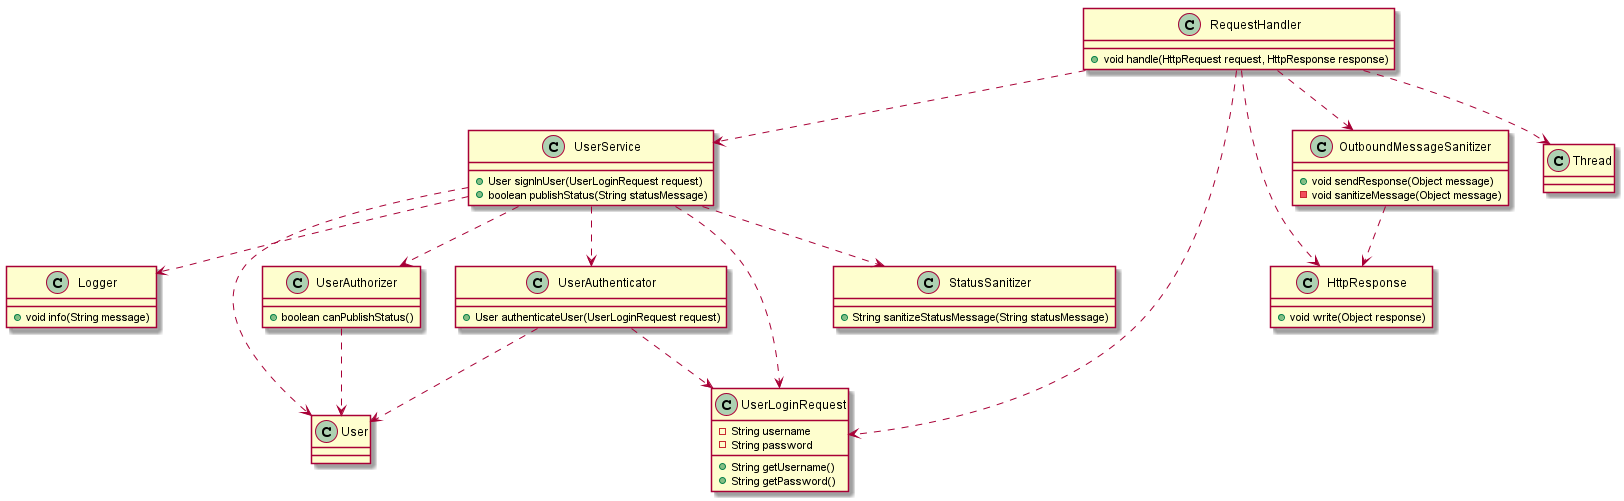
\includegraphics[width=\textwidth]{figure/ToyApp.png}
    \caption{An example of a system, for the purpose of illustrating how the constraints are applied.}
    \label{fig:toy_application}
\end{figure}

\subsection{Enforce AuthN/AuthZ at single point}
% Description
The second constraint is defined in terms of two concepts: an authentication point and an authentication enforcer. Authentication is performed through a method call to the authentication enforcer, which is a class whose sole responsibility is to authenticate an actor. This call should occur at the authentication point, and at no other points in the system, for the sake of ensuring a uniform authentication mechanism throughout the system. Authorization is enforced in the same manner, with the concepts of an authorization point and an authorization enforcer.

% Rule definition
The definition of the second constraint is detailed in Listing~\ref{lst:constraint_2_impl}. The constraint is defined as two separate rules, for the sake of clarity, but their implementations are identical.

\begin{minipage}{\linewidth}
\begin{lstlisting}[caption={Rule definition for constraint 2.}, captionpos=b, label=lst:constraint_2_impl, numbers=left]
ArchRule enforceAuthenticationAtCentralPoint(
        Class<?> authenticationPoint,
        Class<?> authenticator) {
    return CompositeArchRule.of(
        theClass(authenticationPoint)
            .should(callMethod(declaredIn(authenticator)))
    ).and(
        methods()
            .that().areDeclaredIn(authenticator)
            .should(onlyBeAccessedBy(authenticationPoint))
    );
}

ArchRule enforceAuthorizationAtCentralPoint(
        Class<?> authorizationPoint,
        Class<?> authorizer) {
    return enforceAuthenticationAtCentralPoint(
        authorizationPoint,
        authorizer
    );
}
\end{lstlisting}
\end{minipage}

% Applied to toy app
In the example system, the authentication and authorization points are both situated in the \texttt{UserService} class while authentication and authorization are enforced by the classes \texttt{UserAuthenticator} and \texttt{UserAuthorizer} respectively. The application of the rule can be seen in Listing~\ref{lst:constraint_2_toy}.

\begin{minipage}{\linewidth}
\begin{lstlisting}[caption={Application of constraint 2 to the example system.}, captionpos=b, label=lst:constraint_2_toy, numbers=left]
@ArchTest
ArchRule enforceAuthentication = SecArchUnit
    .enforceAuthenticationAtCentralPoint(UserService.class, UserAuthenticator.class);

@ArchTest
ArchRule enforceAuthorization = SecArchUnit
    .enforceAuthorizationAtCentralPoint(UserService.class, UserAuthorizer.class);
\end{lstlisting}
\end{minipage}

\subsection{Messages are sent from a central point}
% Description
The third constraint dictates that all outbound messages are sent from a central sending point. The intent is to have a single point that handles output sanitization or performs other safety checks on messages before they are sent. The act of sending a message is defined as a method call to a sender with at least one argument, which is assumed to contain the message contents. The reasoning is that any class should be allowed to create and pass around a sender instance without violating the constraint.

% Rule definition
The rule definition can be seen in Listing~\ref{lst:constraint_3_impl}. Since there can be multiple sender classes in a system, e.g. one for HTTP requests and one for SMTP messages, the rule accepts a predicate that can select all these sender classes.

\begin{minipage}{\linewidth}
\begin{lstlisting}[caption={Rule definition for constraint 3.}, captionpos=b, label=lst:constraint_3_impl, numbers=left]
ArchRule sendOutboundMessagesFromCentralPoint(
        Class<?> sendingPoint,
        DescribedPredicate<? super JavaClass> senderDescriptor) {
    return methods()
        .that().areDeclaredInClassesThat(senderDescriptor)
        .and(haveAtLeastOneParameter)
        .should(onlyBeAccessedBy(sendingPoint));
}
\end{lstlisting}
\end{minipage}

% Applied to toy app
Listing~\ref{lst:constraint_3_toy} showcases how the constraint can be applied to the example system. In this system, there is a single sender class \texttt{HttpResponse}, responsible for returning a response to a client. The central sending point is the \texttt{OutboundMessageSanitizer} class. 

\begin{minipage}{\linewidth}
\begin{lstlisting}[caption={Application of constraint 3 to the example system.}, captionpos=b, label=lst:constraint_3_toy, numbers=left]
@ArchTest
ArchRule centralSendingPoint = SecArchUnit
    .sendOutboundMessagesFromCentralPoint(
        OutboundMessageSanitizer.class,
        type(HttpResponse.class)
    );
\end{lstlisting}
\end{minipage}




\section{Injecting Information into Source Code}

Some of the architectural constraints require that the developer injects additional information into the source code.

In some cases, this information is simply an indicator that says something about an entire class. Naming the class with a specific suffix is one approach to accomplish this. Another approach is to implement an empty interface, which is the technique used with Java's \texttt{Serializable}\footnote{https://docs.oracle.com/javase/7/docs/api/java/io/Serializable.html} interface. 

In other cases, however, the information may be required for methods of arbitrary signatures and even specific fields. For the purposes of flexibility and minimal obtrusiveness, any extra information is expressed in the form of annotations. These can be applied to classes, fields, methods and parameters without changing the underlying architecture of the system.

\todo{Specific example that requires additional information}

\todo{Show rule definition for each constraint}
\todo{Show how each constraint is used in our toy app}

\subsection{Validate user input}
...

\begin{minipage}{\linewidth}
\begin{lstlisting}[caption={Rule definition for constraint 4.}, captionpos=b, label=lst:constraint_4_impl, numbers=left]
public static ArchRule validateUserInput() {
    return codeUnits()
        .that().areAnnotatedWith(UserInput.class)
        .should(performDirectOrIndirectValidation);
}
\end{lstlisting}
\end{minipage}

\subsection{Restrict thread spawning}
While resources is a broad term, this constraint focuses on preventing the exhaustion of CPU and memory resources through the creation of new threads and processes. As such, every block of code that contains a call to the \texttt{start()} method of a \texttt{Thread}\footnote{https://docs.oracle.com/javase/7/docs/api/java/lang/Thread.html} or any of its subclasses, must be marked as containing a resource restriction mechanism. The same rule is applied for calls to \texttt{ProcessBuilder.start()}\footnote{https://docs.oracle.com/javase/7/docs/api/java/lang/Process.html} and \texttt{Runtime.exec()}\footnotemark[3], which lead to the creation of new processes.
% TODO manual footnote, adjust as necessary

The marking is done with the help of an annotation, either on the relevant method or the entire class. The decision of how the restriction mechanism is implemented is left to the developer of the system.

\begin{minipage}{\linewidth}
\begin{lstlisting}[caption={Rule definition for constraint 5.}, captionpos=b, label=lst:constraint_5_impl, numbers=left]
public static ArchRule limitResourceAllocation() {
    return noClasses()
        .that().areNotAnnotatedWith(ResourceRestriction.class)
        .should().callMethodWhere(
            aThreadIsStartedWithoutRestriction
        ).orShould().callMethodWhere(
            aProcessIsStartedWithoutRestriction
        );
}
\end{lstlisting}
\end{minipage}




\section{Extending ArchUnit Analysis}

In the current ArchUnit API, a rule that aims to constrain access to a method (or field) must be expressed in terms of the type signatures of the source and target methods. Some of our constraints require knowledge about the type signature of the object that is being passed as a parameter. This is a non-issue when fields and method parameters are of the same types as the objects being passed to them. However, in cases where a method signature accepts a "more general" type, such as an \texttt{Object}, there is no way for ArchUnit to constrain the types of the objects that are actually being passed as arguments.

ArchUnit builds its representation of the architecture using ASM\footnote{\url{https://asm.ow2.io/}}, a Java bytecode analysis framework. This framework contains functionality for keeping track of the stack and local variables while analyzing the instructions of a method. With knowledge of the type signatures of the references on the stack at the time of a method call or field assignment, it is possible to determine the type signatures of objects passed as method arguments or an object being assigned to a field. Our extension provides this additional information in ArchUnit's representation of accesses to fields and methods, which the rule definitions can then make use of.

\todo{Specific example that requires an extension}

\subsection{Extensions}

\todo{Detail the extensions we made}

\subsection{Constraints}

\todo{Show rule definition for each constraint}
\todo{Show how each constraint is used in our toy app}

\subsubsection*{Do not allow sensitive information to bleed to other components}
...

\subsubsection*{Do not log secrets}
...


% Validation against open-source systems
\chapter{Evaluation}

This chapter presents an evaluation of the constraints when applied to a number of open source systems. The evaluation was performed in two ways: first a comparison between SecArchUnit and static analysis tools used in industry, and then a standalone evaluation of the tool extension.

\section{Comparison with Industry Tools}
As mentioned in Section~\ref{sec_tools_used_in_comparison}, constraints 1-5 can be validated in both SonarQube and PMD through the definitions of custom rules. The constraints are applied to the test systems presented in Section~\ref{sct:selected-systems} and validated using each of the three tools. Both the relative and absolute frequencies of violations of each constraint can be seen in Figure~\ref{bar:rel_frequency_violation_compraison} and Figure~\ref{bar:frequency_violation_compraison} respectively.

\begin{figure}[h]
  \centering
  \captionsetup{justification=centering}
  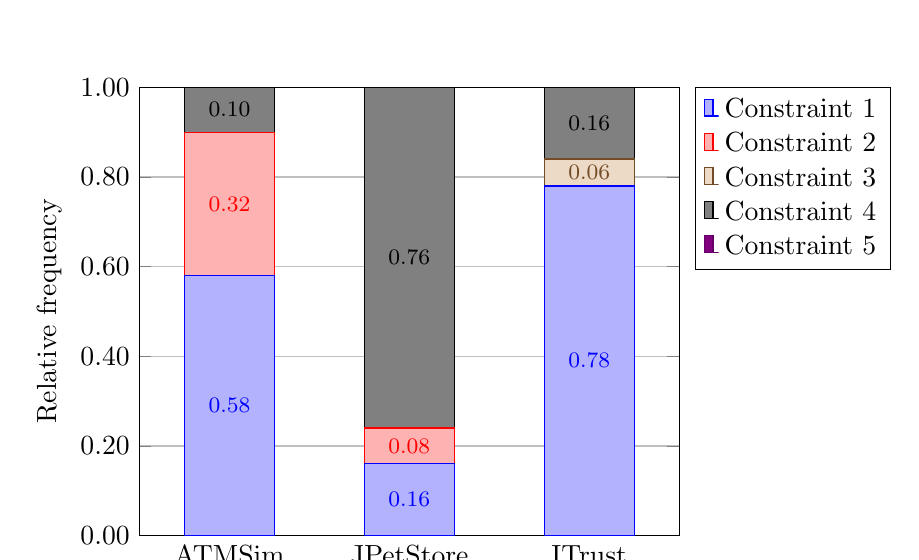
\begin{tikzpicture}\pgfkeys{
     /pgf/number format/precision=2, 
    /pgf/number format/fixed zerofill=true,
    /pgf/number format/fixed
}
  
    \begin{axis}[
        ybar stacked,
        ymajorgrids = true,
        nodes near coords,
        every node near coord/.append style={font=\footnotesize},
        xbar legend,
%         nodes near coords align={right},
        legend pos=outer north east,
        enlarge x limits=0.25,
        enlarge y limits=false,
        bar width=.5,
        % x axis
        xtick={1,2,3},
        xticklabels={ATMSim,JPetStore,ITrust},
        %x tick label style={rotate=45,anchor=east},
        % y axis
        ymin=0,
        ylabel={Relative frequency},
      ]
     % C1
     \addplot+[ybar] plot coordinates {(1,0.58) (2,0.16) 
      (3,0.78)};
     % C2
    \addplot+[ybar] plot coordinates {(1,0.32) (2,0.08) 
      (3,0)};
     % C3
    \addplot+[ybar] plot coordinates {(1,0) (2,0)
      (3,0.06)};
     % C4
    \addplot+[ybar] plot coordinates {(1,0.1) (2,0.76) 
      (3,0.16)};
     % C5
    \addplot+[ybar] plot coordinates {(1,0) (2,0) 
      (3,0)};
      

      \legend{Constraint 1,Constraint 2,Constraint 3, Constraint 4, Constraint 5}
    \end{axis}
  \end{tikzpicture}

  \caption{The relative frequency of constraint violations found in the three projects.}
  \label{bar:rel_frequency_violation_comparison}
\end{figure}
\begin{figure}
\centering
\captionsetup{justification=centering}

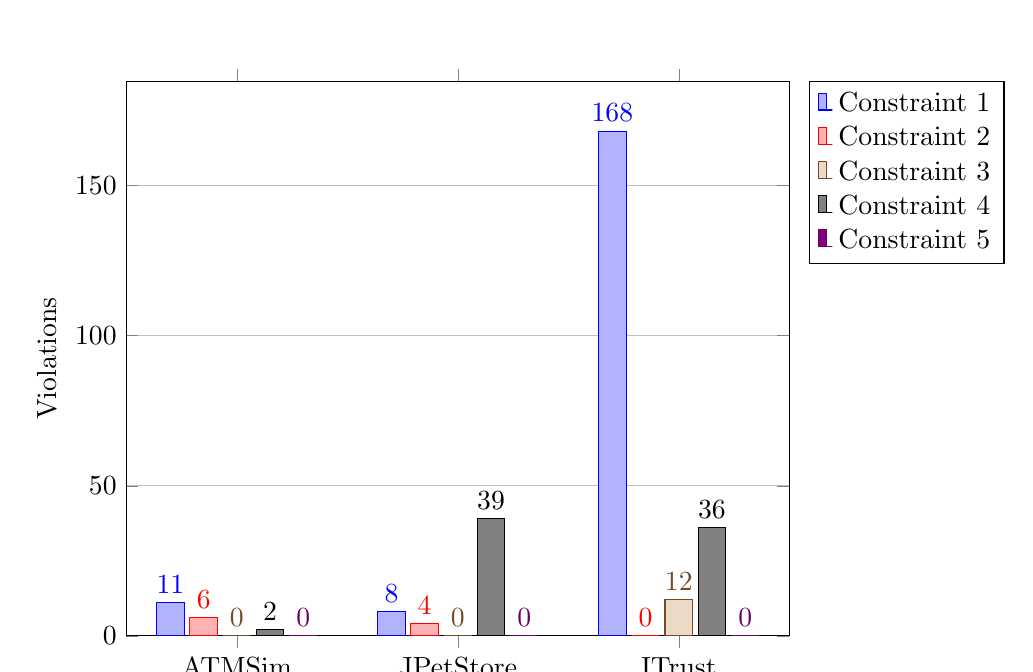
\begin{tikzpicture}
\begin{axis}[
    width=10cm,
    ybar,
    ymin = 0,
    ymajorgrids = true,
    enlarge x limits=0.25,
    xbar legend,
    legend pos=outer north east,
    ylabel={Violations},
    symbolic x coords={ATMSim,JPetStore,ITrust},
    %xlabel={System},
    xtick=data,
    nodes near coords,
    nodes near coords align={vertical},
    ]
%C1
\addplot coordinates {(ATMSim,11) (JPetStore,8) (ITrust,168)};
%C2
\addplot coordinates {(ATMSim,6) (JPetStore,4) (ITrust,0)};
%C3
\addplot coordinates {(ATMSim,0) (JPetStore,0) (ITrust,12)};
%C3
\addplot coordinates {(ATMSim,2) (JPetStore,39) (ITrust,36)};
%C3
\addplot coordinates {(ATMSim,0) (JPetStore,0) (ITrust,0)};
\legend{Constraint 1,Constraint 2,Constraint 3, Constraint 4, Constraint 5}
\end{axis}
\end{tikzpicture}

\caption{The constraint violations found in the ground truth of each system.}
\label{bar:frequency_violation_comparison}
\end{figure}

As shown in the figures, the systems were evaluated using imbalanced data. Constraint 1 accounted for a majority of all violations found throughout all three systems, while no system violated constraint 5. Addtionally, iTrust where the only system to contain a violation of constraint 3. 

Each tool is evaluated according to the selected performance metrics, i.e. precision and recall. These results are presented in Table~\ref{tab:results_comparison}. Both in regards to precision, as well as recall, the tools performed equally. However, the causes of failure, in cases where the results of the tools varied, differed noticeably. The examples are described below:

\begin{itemize}
    \item In ATM simulator, the same false positive occurred in all three tools. This was related to constraint 3, where a subclass of the sending point contained a method call to the sender. Additionally, PMD had 4 false negatives which occurred because it was unable to determine the classes that these method calls targeted.
    \item In JPetStore, PMD reported 4 false negatives, again because it was unable to determine the target class of these method calls.
    \item In iTrust, a security service contained both an inner interface and inner class whose methods did not perform security events. Both PMD and SonarQube analyzes the AST with a single class as its root node, thus they consider the inner members to be separate objects of analysis. In comparison, ArchUnit uses the entire Java file in its analysis causing it to incorrectly apply the annotation of the outer class to the inner members. 
\end{itemize}

\newcolumntype{g}{>{\columncolor{RowColor}}c}
\newcolumntype{x}{>{\columncolor{RowColor}}l}
\begin{table}[h]
\begin{center}
\begin{tabular}{lxggggg}
\rowcolor{white}
\textbf{Project}           & \textbf{Tool}    & \textbf{TP} & \textbf{FP} & \textbf{FN} & \textbf{Precision} & \textbf{Recall} \\
\hline
\rowcolor{white}
\multirow[t]{3}{*}{ATMsim}    & SecArchUnit      & 19          & 1           & 0           & 1               & 0.95            \\
                           & SonarQube Plugin & 19          & 1           & 0           & 1               & 0.95            \\
                           \rowcolor{white}
                           & PMD Plugin       & 15          & 1           & 4           & 0.94               & 0.79            \\
\hline
\rowcolor{white}
\multirow[t]{3}{*}{JPetStore} & SecArchUnit      & 51          & 0           & 0           & 1                  & 1               \\
                           & SonarQube Plugin & 51          & 0           & 0           & 1                  & 1               \\
                           \rowcolor{white}
                           & PMD Plugin       & 47          & 0           & 4           & 1                  & 0.92            \\
\hline
\rowcolor{white}
\multirow[t]{3}{*}{ITrust}    & SecArchUnit      & 216         & 3           & 0           & 0.97               & 1               \\
                           & SonarQube Plugin & 216         & 0           & 0           & 1                  & 1               \\
                           \rowcolor{white}
                           & PMD Plugin       & 216         & 0           & 0           & 1                  & 1 \\
\hline
\end{tabular}
\end{center}
\caption{Results from validating constraints 1-5 using SecArchUnit, SonarQube and PMD.}
\label{tab:results_comparison}
\end{table}

\section{Validation of ArchUnit Extension}
Constraints 6-7, which rely on an extension of ArchUnit's analysis, are validated solely using SecArchUnit. The performance metrics from applying the final two constraints to iTrust are presented in Table~\ref{tab:tool_extension}.

The system, iTrust, initially contained no violations of constraint 7. Therefore, violations were injected by systematically marking all identifier fields (e.g. \texttt{patientId}, \texttt{personnelId}) in the model and base-action packages as secrets. We chose to mark these identifiers because they were commonly sent to the logger as a way to describe the patient or personnel involved in a transaction. Hence, the 37 violations of constraint 7, as seen in Table~\ref{tab:tool_extension}, are artificially injected.

Moreover, iTrust is built with a mix of Java and Java Server Pages (JSP) files whereas ArchUnit can only analyze Java bytecode. The classes in the action package, from which the logger is called, are all instantiated in the JSP files outside the view of our analysis. As such, the types of information flow that are analyzed and included in the ground truth are rather rudimentary. Out of the 37 violations of constraint 7, 1 was found without recursion (direct access to secret field) and the remaining 36 were found using a single recursion step (access to getter method of a secret field).
% This is bad - we could just as well put the secret annotation on the getter and enforce the same cases in SonarQube/PMD

\begin{table}
\begin{center}
\begin{tabular}{lccccc}
\hline
\textbf{Constraint} & \textbf{TP} & \textbf{FP} & \textbf{FN} & \textbf{Precision} & \textbf{Recall} \\
\hline
6 & 24 & 0 & 0 & 1 & 1\\
\rowcolor{RowColor}
7 & 37 & 0 & 0 & 1 & 1\\
\hline
\end{tabular}
\end{center}
\caption{Results from validating the extension-based constraints on iTrust.}
\label{tab:tool_extension}
\end{table}

% CONCLUSION
% CREATED BY DAVID FRISK, 2018
\chapter{Conclusion}




% REFERENCES / BIBLIOGRAPHY
\cleardoublepage
\addcontentsline{toc}{chapter}{Bibliography}
\bibliographystyle{IEEEtran}
\bibliography{references}

% APPENDICES
\cleardoublepage
\appendix
\setcounter{page}{1}
\pagenumbering{Roman}			% Capitalized roman numbering starting from I (one)

\chapter{Ground Truth Tables}\label{chap:groundtruth}

This appendix contains an excerpt of our ground truth focusing soley on the ATMSimulator system. The entriety of the data can be found in our public repository\footnote{\url{https://github.com/MarcusRandevik/SecArchUnit/blob/master/Validation/Validation.xlsx}}. 

The data presented here consists of three tables:

\begin{itemize}
    \item Table~\ref{tab:groundtruthviolations} contains the identified violations of all constrains in ATMSimulator. It is this data that the tools were evaluated against.
    \item Table~\ref{tab:groundtruthconceptincluded} contains the concepts of our constraints that were applied to the target system. These were later used to identify the violations of constraints in Table~\ref{tab:groundtruthviolations}.
    \item Finally, Table~\ref{tab:groundtruthconceptnotincluded} presents concepts that were considered by at least one author but later discarded and not included when forming the ground truth. 
\end{itemize}  

\begin{table}[ht]
\captionsetup{justification=centering}
\caption{Table of constraints violations found within ATMSimulator.}
\hspace*{-1.6cm}
\label{tab:groundtruthviolations}
\begin{center}
\begin{tabular}{llllll}
\textbf{Marcus}   & \textbf{Patrik}   & \textbf{Conclusion} & \textbf{Constraint} & \textbf{Class} & \textbf{Line} \\
\hline
POSITIVE & NEGATIVE & POSITIVE   & 1          & CardReader     & 40       \\
\rowcolor{RowColor}
POSITIVE & NEGATIVE & POSITIVE   & 1          & CardReader     & 47       \\
POSITIVE & NEGATIVE & POSITIVE   & 1          & CardReader     & 55       \\
\rowcolor{RowColor}
POSITIVE & POSITIVE & POSITIVE   & 1          & CashDispenser  & 35       \\
POSITIVE & POSITIVE & POSITIVE   & 1          & CashDispenser  & 45       \\
\rowcolor{RowColor}
POSITIVE & POSITIVE & POSITIVE   & 1          & NetworkToBank  & 37       \\
POSITIVE & POSITIVE & POSITIVE   & 1          & NetworkToBank  & 44       \\
\rowcolor{RowColor}
POSITIVE & POSITIVE & POSITIVE   & 1          & Transaction & 56       \\
POSITIVE & POSITIVE & POSITIVE   & 1          & Transaction & 96       \\
\rowcolor{RowColor}
POSITIVE & POSITIVE & POSITIVE   & 1          & Transaction & 219      \\
POSITIVE & POSITIVE & POSITIVE   & 1          & Transaction & 258      \\
\rowcolor{RowColor}
POSITIVE & POSITIVE & POSITIVE   & 2          & Receipt             & 41       \\
POSITIVE & POSITIVE & POSITIVE   & 2          & Session                 & 76       \\
\rowcolor{RowColor}
POSITIVE & POSITIVE & POSITIVE   & 2          & Session                 & 90       \\
POSITIVE & POSITIVE & POSITIVE   & 2          & Receipt             & 41       \\
\rowcolor{RowColor}
POSITIVE & POSITIVE & POSITIVE   & 2          & Session                 & 76       \\
POSITIVE & POSITIVE & POSITIVE   & 2          & Session                 & 90       \\
\rowcolor{RowColor}
POSITIVE & POSITIVE & POSITIVE   & 4          & CardReader     & 40       \\
POSITIVE & POSITIVE & POSITIVE   & 4          & OperatorPanel  & 39     \\
\hline
\end{tabular}
\end{center}
\end{table}

\begin{table}
\begin{center}
\captionsetup{justification=centering}
\caption{Table of concepts mapped to classes within ATMSimulator, both in initial agreement and disagrement. These are later used to find violations as presented in Table~\ref{tab:groundtruthviolations}.}
\label{tab:groundtruthconceptincluded}
\hspace*{-2.7cm}
\begin{tabular}{p{3.5cm}p{3.5cm}p{3.5cm}ll}
\textbf{Marcus} & \textbf{Patrik} & \textbf{Conclusion} & \textbf{Cons} & \textbf{Class/Member} \\
\hline
Class not considered as security service & Class considered as security service & The public methods were considered as a security service as they are the entry point to a crucial set of operations & 1                   & CardReader                     \\
\rowcolor{RowColor}
Class considered as security service     & Class considered as security service & -                                                                                                              & 1                   & CashDispenser                  \\
Class considered as security service     & Class considered as security service & -                                                                                                              & 1                   & NetworkToBank                  \\
\rowcolor{RowColor}
Class considered as security service     & Class considered as security service & -                                                                                                              & 1                   & Transaction                 \\
Authenticator                            & Authenticator                        & -                                                                                                              & 2                   & Transaction                 \\
\rowcolor{RowColor}
Central sender                           & Central Sender                       & -                                                                                                              & 3                   & NetworkToBank                  \\
Sending point                            & Sending point                        & -                                                                                                              & 3                   & Transaction                 \\
\rowcolor{RowColor}
User Input                               & User Input                           & -                                                                                                              & 4                   & CardReader.readCard            \\
User Input                               & User Input                           & -                                                                                                              & 4                   & CustomerConsole.readPin        \\
\rowcolor{RowColor}
User Input                               & User Input                           & -                                                                                                              & 4                   & CustomerConsole.readMenuChoice \\
User Input                               & User Input                           & -                                                                                                              & 4                   & CustomerConsole.readAmount     \\
\rowcolor{RowColor}
User Input                               & User Input                           & -                                                                                                              & 4                   & OperatorPanel.getInitialCash   \\
Input validator                          & Input validator                      & -                                                                                                              & 4                   & CustomerConsole.readPin        \\
\rowcolor{RowColor}
Input validator                          & Input validator                      & -                                                                                                              & 4                   & CustomerConsole.readMenuChoice \\
Input validator                          & Input validator                      & -                                                                                                              & 4                   & CustomerConsole.readAmount     \\
\rowcolor{RowColor}
ResourceRestriction                      & ResourceRestriction                  & -                                                                                                              & 5                   & ATMApplet                                   \\
ResourceRestriction                      & ResourceRestriction                  & -                                                                                                              & 5                   & ATMMain  \\
\hline
\end{tabular}
\end{center}
\end{table}

\begin{sidewaystable}
\begin{center}
\captionsetup{justification=centering}
\caption{Table of concepts that were considered by at least one author but later discarded.}
\label{tab:groundtruthconceptnotincluded}
\hspace*{-2cm}
\begin{tabular}{p{4cm}p{4cm}p{6cm}ll}
\textbf{Marcus} & \textbf{Patrik} & \textbf{Conclusion} & \textbf{Constraint} & \textbf{Class} \\
\hline
Class considered as security service & Class not considered as security service & Not a security service as it is the loop at which other components act & 1 & Session \\
\rowcolor{RowColor}
Class considered to be out of system domain & Class considered to be authentication point and enforcer & The class represents the simulated functionality of a bank, thus being outside of the system. Class will not be considered as authentication point/enforcer & 2 & SimulatedBank \\
\hline
\end{tabular}
\end{center}
\end{sidewaystable}
\chapter{BlogWeb} \label{apx:blogweb}

See full-scale UML diagram on the next page.

\begin{sidewaysfigure}
    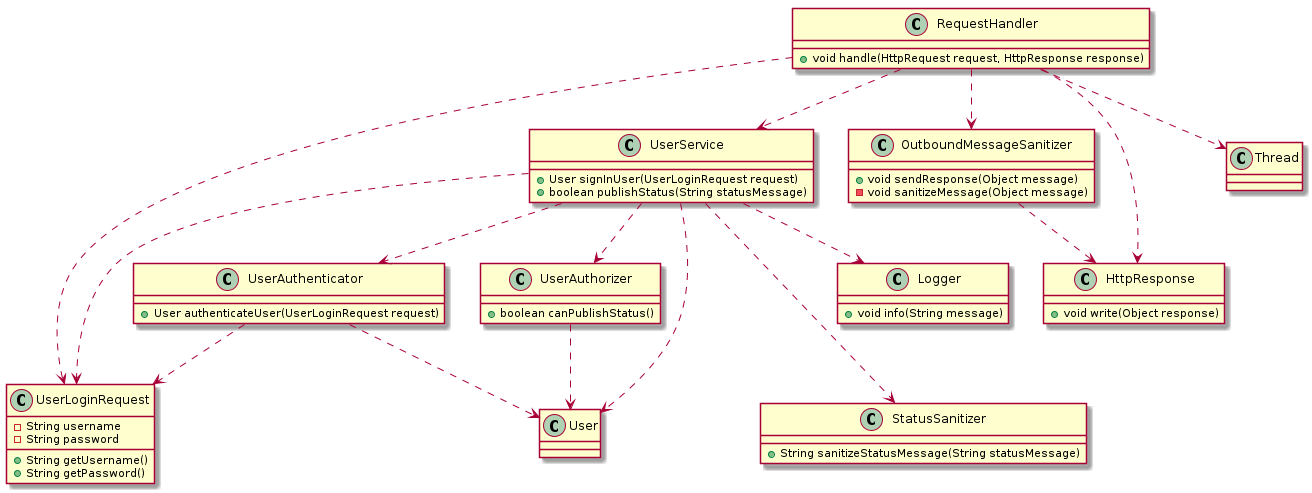
\includegraphics[width=\textwidth]{figure/ToyAppFull.png}
    \captionsetup{justification=centering}
    \caption
        [UML class diagram of the toy system BlogWeb]
        {A UML class diagram of the toy system BlogWeb.}
\end{sidewaysfigure}
\chapter{SecArchUnit Code Excerpts}
\begin{lstlisting}[caption=Constraint 4: performDirectOrIndirectValidation custom condition., captionpos=b, label=lst:constraint_4_condition, numbers=left, showstringspaces=false]
ArchCondition<JavaCodeUnit> performDirectOrIndirectValidation =
new ArchCondition<>("perform direct or indirect validation") {
  @Override
  void check(JavaCodeUnit codeUnit, ConditionEvents events) {
    if (codeUnit.isAnnotatedWith(InputValidator.class)) {
      // Validates input directly => condition passed
      return;
    }

    boolean callsValidator = codeUnit.getCallsFromSelf().stream()
      .map(call -> call.getTarget())
      .anyMatch(target -> 
        target.isAnnotatedWith(InputValidator.class)
        || target.getOwner().isAnnotatedWith(InputValidator.class)
      );
    if (callsValidator) {
      // Calls a validator => condition passed
      return;
    }

    boolean calledAtLeastOnce = !codeUnit.getAccessesToSelf()
      .isEmpty();
    boolean onlyCalledByValidators = codeUnit.getAccessesToSelf()
      .stream()
      .map(call -> call.getOrigin())
      .allMatch(origin -> origin.isAnnotatedWith(InputValidator.class)
        || origin.getOwner().isAnnotatedWith(InputValidator.class));
    if (calledAtLeastOnce && onlyCalledByValidators) {
      // Is only called by validators => condition passed
      return;
    }

    String message = codeUnit.getFullName() + " takes user input that is never validated";
    events.add(SimpleConditionEvent.violated(codeUnit, message));
  }
};
\end{lstlisting}

\begin{lstlisting}[caption=Constraint 5: \texttt{aThreadIsStartedWithoutRestriction} custom predicate., captionpos=b, label=lst:constraint_5_predicate_1, numbers=left, showstringspaces=false]
DescribedPredicate<JavaMethodCall> aThreadIsStartedWithoutRestriction =
new DescribedPredicate<>("a thread is started") {
    @Override
    public boolean apply(JavaMethodCall call) {
        AccessTarget.MethodCallTarget target = call.getTarget();

        boolean isRestricted = call.getOrigin()
            .isAnnotatedWith(ResourceRestriction.class);
        boolean startsAThread = 
            target.getOwner().isAssignableTo(Thread.class)
            && target.getName().equals("start");

        return !isRestricted && startsAThread;
    }
};
\end{lstlisting}

\begin{lstlisting}[caption=Constraint 5: \texttt{aProcessIsStartedWithoutRestriction} custom predicate., captionpos=b, label=lst:constraint_5_predicate_2, numbers=left, showstringspaces=false]
DescribedPredicate<JavaMethodCall> aProcessIsStartedWithoutRestriction =
new DescribedPredicate<>("a process is started") {
    @Override
    public boolean apply(JavaMethodCall call) {
        AccessTarget.MethodCallTarget target = call.getTarget();

        boolean isRestricted = call.getOrigin()
            .isAnnotatedWith(ResourceRestriction.class);
        boolean startsAProcess =
            target.getOwner().isEquivalentTo(ProcessBuilder.class)
                && target.getName().equals("start")
            || target.getOwner().isEquivalentTo(Runtime.class)
                && target.getName().equals("exec");

        return !isRestricted && startsAProcess;
    }
};
\end{lstlisting}

\clearpage
\begin{lstlisting}[caption=Constraint 6: \texttt{notBleedToInsecureComponents} custom condition., captionpos=b, label=lst:constraint_6_condition, numbers=left, showstringspaces=false]
ArchCondition<JavaField> notBleedToInsecureComponents =
new ArchCondition<>("not bleed to insecure components") {
    @Override
    public void check(JavaField field, ConditionEvents events) {
        // Direct access
        field.getAccessesToSelf().stream()
            .filter(access -> !access.getOriginOwner()
                .isAnnotatedWith(AssetHandler.class))
            .forEach(offendingFieldAccess -> {
                String message = offendingFieldAccess
                    + ": access to asset " + field.getName();
                events.add(SimpleConditionEvent.violated(offendingFieldAccess, message));
            });

        // Access via getter method
        field.getAccessesToSelf().stream()
            .filter(access -> access.getOrigin() instanceof JavaMethod)
            .map(access -> (JavaMethod) access.getOrigin())
            .filter(method ->
                method.getReturnValueHints().stream()
                    .anyMatch(hint ->
                        field.equals(hint.getMemberOrigin())
                    )
                )
            .flatMap(method -> method.getCallsOfSelf().stream())
            .filter(call -> !call.getOriginOwner()
                .isAnnotatedWith(AssetHandler.class))
            .forEach(offendingMethodCall -> {
                String message = offendingMethodCall
                    + ": access to asset " + field.getName()
                    + " (via getter method)";
                events.add(SimpleConditionEvent.violated(offendingMethodCall, message));
            });
    }
};
\end{lstlisting}

\clearpage
\begin{lstlisting}[caption=Constraint 7: \texttt{passSecretArgumentTo} custom condition., captionpos=b, label=lst:constraint_7_condition, numbers=left, showstringspaces=false]
ArchCondition<JavaClass> passSecretArgumentTo(
    DescribedPredicate<JavaAccess<?>> target) {
return new ArchCondition<>("pass @Secret argument to "
    + target.getDescription()) {
  @Override
  public void check(JavaClass clazz, ConditionEvents events) {
    clazz.getMethodCallsFromSelf().stream()
      .filter(call -> target.apply(call))
      .forEach(callToTarget -> {
        InformationFlow.recurseOnHints(
            callToTarget.getArgumentHints()
          )
          .filter(hint -> hint.getMemberOrigin() != null)
          .map(hint -> hint.getMemberOrigin())
          .filter(member ->
            member.isAnnotatedWith(Secret.class)
            || member.getOwner().isAnnotatedWith(Secret.class)
          )
          .distinct()
          .forEach(secretMember -> {
            String message = callToTarget.getSourceCodeLocation()
              + " passes secret "
              + secretMember.getOwner().getSimpleName()
              + "." + secretMember.getName();
            events.add(SimpleConditionEvent.satisfied(
              callToTarget,
              message)
            );
          });
      });
  }
};
\end{lstlisting}

\clearpage
\begin{lstlisting}[caption=Constraint 7: \texttt{InformationFlow} class used for hint recursion., captionpos=b, label=lst:constraint_7_flow, numbers=left, showstringspaces=false]
class InformationFlow {
    Stream<Hint> recurseOnHints(Set<Hint> hints) {
        return recurseOnHints(hints, 5).distinct();
    }

    Stream<Hint> recurseOnHints(Set<Hint> hints, int depth) {
        if (depth == 0 || hints.isEmpty()) {
            return hints.stream();
        }

        // Hints with an originating member
        Set<JavaMember> hintOrigins = hints.stream()
            .filter(hint -> hint.getMemberOrigin() != null)
            .map(hint -> hint.getMemberOrigin())
            .collect(Collectors.toSet());

        // Hints flowing into a field
        Stream<Hint> hintsFlowingIntoFields = hintOrigins.stream()
            .filter(member -> member instanceof JavaField)
            .map(member -> (JavaField) member)
            .flatMap(hint -> hint.getAccessesToSelf().stream())
            .flatMap(access -> access.getArgumentHints().stream());

        // Hints flowing out of a method
        Stream<Hint> hintsFlowingOutOfMethods = hintOrigins.stream()
            .filter(member -> member instanceof JavaMethod)
            .map(member -> (JavaMethod) member)
            .flatMap(method -> method.getReturnValueHints().stream());

        // Collect hints from this level
        Set<Hint> recursedHints = Stream.concat(
                hintsFlowingIntoFields, 
                hintsFlowingOutOfMethods
            )
            .collect(Collectors.toSet());

        // Concatenate this level of hints with the next recursion level
        return Stream.concat(hints.stream(), recurseOnHints(recursedHints, depth - 1));
    }
}
\end{lstlisting}
\chapter{SonarQube Rule Definitions}
\label{apx:sonarqube}

\begin{lstlisting}[caption={Constraint 1.}, captionpos=b, label=lst:sq_1, numbers=left, showstringspaces=false]
public class LogSecurityEventsRule
    extends IssuableSubscriptionVisitor {

  public static String LOGGER_CLASS = "edu.ncsu.csc.itrust.action.EventLoggingAction";
  public static List<String> SECURITY_CLASSES = Arrays.asList(
      "ActivityFeedAction".toLowerCase(),
  );

  MethodMatchers loggerMethods = MethodMatchers.create()
    .ofTypes(LOGGER_CLASS).anyName().withAnyParameters()
    .build();

  @Override
  public List<Tree.Kind> nodesToVisit() {
    return Collections.singletonList(Tree.Kind.METHOD);
  }

  @Override
  public void visitNode(Tree tree) {
    MethodTree method = (MethodTree) tree;

    String methodEnclosingClass = method.symbol().enclosingClass()
      .name().toLowerCase();
    if (!SECURITY_CLASSES.contains(methodEnclosingClass)) {
      // Method not defined in a security service => skip
      return;
    }

    boolean isPublicMethod = false;
    for (ModifierKeywordTree keywordTree : method.modifiers().modifiers()) {
      if (keywordTree.modifier() == Modifier.PUBLIC) {
        isPublicMethod = true;
        break;
      }
    }

    if (!isPublicMethod) {
      // Not a public method => skip
      return;
    }

    boolean containsCallToLogger = false;

    ControlFlowGraph cfg = method.cfg();

    for (ControlFlowGraph.Block block : cfg.blocks()) {
      for (Tree blockTree : block.elements()) {
        if (blockTree.is(Tree.Kind.METHOD_INVOCATION)) {
          MethodInvocationTree mit = (MethodInvocationTree) blockTree;
          if (loggerMethods.matches(mit)) {
            // 
            containsCallToLogger = true;
          }
        }
      }
    }

    if (!containsCallToLogger) {
      reportIssue(method.simpleName(), "Secure classes must contain call to logger");
    }
  }
}
\end{lstlisting}

\begin{lstlisting}[caption={Constraint 2. This rule ensures that at least one method in the authentication point calls the authentication enforcer.}, captionpos=b, label=lst:sq_2, numbers=left, showstringspaces=false]
public class AuthSingleComponentRule
    extends IssuableSubscriptionVisitor {

  private static final String AUTH_POINT_CLASS =
    "OrderActionBean".toLowerCase();
  private static final String AUTH_ENFORCER_CLASS =
    "org.mybatis.jpetstore.web.actions.OrderActionBean";

  private final MethodMatchers authMethods =
    MethodMatchers.create()
    .ofTypes(AUTH_ENFORCER_CLASS).anyName().withAnyParameters()
    .build();

  private static final int INITIAL_AMOUNT_OF_METHODS = -1;
  private int methodsInAuthPoint = INITIAL_AMOUNT_OF_METHODS;
  private int methodsVisited = 0;
  private boolean containsCallToEnforcer = false;

  @Override
  public List<Tree.Kind> nodesToVisit() {
    return Collections.singletonList(Tree.Kind.METHOD);
  }

  @Override
  public void visitNode(Tree tree) {
    MethodTree method = (MethodTree) tree;

    String enclosingClassName = method.symbol().enclosingClass()
      .name().toLowerCase();
    // Check if we're in the auth point class
    if (!AUTH_POINT_CLASS.equals(enclosingClassName)) {
      return;
    }

    methodsVisited++;

    // If this is the first time we're in the auth point class, calculate the number of methods
    if (methodsInAuthPoint == INITIAL_AMOUNT_OF_METHODS) {
      Collection<Symbol> symbols = method.symbol().enclosingClass()
        .memberSymbols();
      setMethodsInAuthPoint(symbols);
    }

    // From the cgf, see if the methods contains a call to enforcer class
    ControlFlowGraph cfg = method.cfg();

    for (ControlFlowGraph.Block block : cfg.blocks()) {
      for (Tree blockTree : block.elements()) {
        if (blockTree.is(Tree.Kind.METHOD_INVOCATION)) {
          MethodInvocationTree mit =
            (MethodInvocationTree) blockTree;
          if (authMethods.matches(mit)) {
            containsCallToEnforcer = true;
          }
        }
      }
    }

    if (methodsVisited >= methodsInAuthPoint
        && !containsCallToEnforcer) {
      reportIssue(
        method.symbol().enclosingClass().declaration(),
        "Authpoint must contain call to enforcer"
      );
    }
  }

  /**
   * Calculate the amount of methods in the authpoint class
   * @param symbols the collection of symbols defined within the authpoint class
   */
  private void setMethodsInAuthPoint(Collection<Symbol> symbols) {
    for (Symbol symbol : symbols) {
      if (symbol.isMethodSymbol() 
          && !symbol.name().equals("<init>")) {
        if (methodsInAuthPoint == INITIAL_AMOUNT_OF_METHODS) {
          methodsInAuthPoint = 1;
        } else {
          methodsInAuthPoint++;
        }
      }
    }

    if (methodsInAuthPoint == INITIAL_AMOUNT_OF_METHODS) {
      methodsInAuthPoint = 0;
    }
  }
}
\end{lstlisting}

\begin{lstlisting}[caption={Constraint 2. This rule ensures that calls to the authentication enforcer only occur in the authentication point.}, captionpos=b, label=lst:sq_2b, numbers=left, showstringspaces=false]
public class AuthSingleComponentEnforcerRule
    extends IssuableSubscriptionVisitor {
  private static final String AUTH_POINT_CLASS =
    "OrderActionBean".toLowerCase();
  private static final String AUTH_ENFORCER_CLASS =
    "org.mybatis.jpetstore.web.actions.OrderActionBean";

  private final MethodMatchers enforcerMethods =
    MethodMatchers.create()
    .ofTypes(AUTH_ENFORCER_CLASS).anyName().withAnyParameters()
    .build();

  @Override
  public List<Tree.Kind> nodesToVisit() {
    return Collections.singletonList(Tree.Kind.METHOD_INVOCATION);
  }

  @Override
  public void visitNode(Tree tree) {
    MethodInvocationTree mit = (MethodInvocationTree) tree;

    if (enforcerMethods.matches(mit)) {
      // Get the class of the calling method
      Tree parent = mit.parent();
      while (!parent.is(Tree.Kind.CLASS)) {
        parent = parent.parent();
      }
      ClassTree classTree = (ClassTree) parent;
      String enclosingClassOfCaller = classTree.symbol()
        .name().toLowerCase();

      if (!AUTH_POINT_CLASS.equals(enclosingClassOfCaller)) {
        reportIssue(mit, "Method invocation to enforcer must be performed at auth points");
      }
    }
  }
}

\end{lstlisting}

\begin{lstlisting}[caption={Constraint 3.}, captionpos=b, label=lst:sq_3, numbers=left, showstringspaces=false]
class CentralMessageRule extends IssuableSubscriptionVisitor {
  private static final String SENDING_POINT = "Transaction";
  private static final MethodMatchers SENDERS =
    MethodMatchers.create()
    .ofTypes("atm.physical.NetworkToBank")
    .anyName()
    .addParametersMatcher(parameters -> !parameters.isEmpty())
    .build();

  @Override
  public List<Tree.Kind> nodesToVisit() {
    return Collections.singletonList(Tree.Kind.METHOD_INVOCATION);
  }

  @Override
  public void visitNode(Tree tree) {
    MethodInvocationTree methodInvocation =
      (MethodInvocationTree) tree;

    if (SENDERS.matches(methodInvocation)) {
      // Get class where method invocation takes place
      Tree parent = methodInvocation.parent();
      while (!parent.is(Tree.Kind.CLASS)) {
        parent = parent.parent();
      }
      ClassTree classTree = (ClassTree) parent;

      // Compare class with sending point
      String sendingClassName = classTree.symbol().name();
      if (!SENDING_POINT.equals(sendingClassName)) {
        reportIssue(methodInvocation, "Messages must only be sent from the sending point");
      }
    }
  }
}
\end{lstlisting}

\begin{lstlisting}[caption={Constraint 4.}, captionpos=b, label=lst:sq_4, numbers=left, showstringspaces=false]
public class ValidateUserInputRule
    extends IssuableSubscriptionVisitor {
  private static final String USER_INPUT =
    "com.github.secarchunit.concepts.UserInput";
  private static final String INPUT_VALIDATOR =
    "com.github.secarchunit.concepts.InputValidator";

  @Override
  public List<Tree.Kind> nodesToVisit() {
    return Collections.singletonList(Tree.Kind.METHOD);
  }

  @Override
  public void visitNode(Tree tree) {
    MethodTree methodTree = (MethodTree) tree;

    // Check if this method deals with user input
    if (!methodTree.symbol().metadata()
        .isAnnotatedWith(USER_INPUT)) {
      return;
    }

    // Check for in-line validation (case 1)
    if (methodTree.symbol().metadata()
        .isAnnotatedWith(INPUT_VALIDATOR)) {
      return;
    }

    // Check for calls to validator (case 2)
    for (Block block : methodTree.cfg().blocks()) {
      for (Tree blockTree : block.elements()) {
        if (blockTree.is(Tree.Kind.METHOD_INVOCATION)) {
          MethodInvocationTree mit = (MethodInvocationTree) blockTree;
          if (mit.symbol().metadata()
              .isAnnotatedWith(INPUT_VALIDATOR)
            || mit.symbol().enclosingClass().metadata()
              .isAnnotatedWith(INPUT_VALIDATOR)) {
            return;
          }
        }
      }
    }

    // Check if all callers are marked as validators (case 3)
    boolean hasCallers = !methodTree.symbol().usages().isEmpty();
    if (hasCallers) {
      boolean validatedInAllCallers = true;

      for (IdentifierTree caller : methodTree.symbol().usages()) {
        if (caller.symbol().metadata()
            .isAnnotatedWith(INPUT_VALIDATOR)) {
          // Caller method is validator
          continue;
        }

        if (caller.symbol().enclosingClass().metadata()
            .isAnnotatedWith(INPUT_VALIDATOR)) {
          // Caller class is validator
          continue;
        }

        validatedInAllCallers = false;
        break;
      }

      if (validatedInAllCallers) {
        return;
      }
    }

    reportIssue(methodTree, "User input must be validated");
  }
}
\end{lstlisting}

\begin{lstlisting}[caption={Constraint 5.}, captionpos=b, label=lst:sq_5, numbers=left, showstringspaces=false]
public class LimitThreadSpawnRule
    extends IssuableSubscriptionVisitor {
  private static final String RESOURCE_RESTRICTION =
    "com.github.secarchunit.concepts.ResourceRestriction";

  private final MethodMatchers threadStartMethods =
    MethodMatchers.create()
      .ofSubTypes("java.lang.Thread").names("start")
      .withAnyParameters().build();
  private final MethodMatchers processStartMethods =
    MethodMatchers.or(
      MethodMatchers.create()
        .ofTypes("java.lang.ProcessBuilder")
        .names("start").withAnyParameters()
        .build(),
      MethodMatchers.create()
        .ofTypes("java.lang.Runtime").names("exec")
        .withAnyParameters()
        .build()
    );

  @Override
  public List<Tree.Kind> nodesToVisit() {
    return Collections.singletonList(Tree.Kind.METHOD);
  }

  @Override
  public void visitNode(Tree tree) {
    MethodTree methodTree = (MethodTree) tree;

    if (methodTree.symbol().isAbstract()) {
      // Skip abstract methods, as they have no code block
      return;
    }

    if (methodStartsThreadOrProcess(methodTree)) {
      // Check for resource restriction marker...
      // ... on method
      if (methodTree.symbol().metadata()
          .isAnnotatedWith(RESOURCE_RESTRICTION)) {
        return;
      }

      // ... or on class
      if (methodTree.symbol().enclosingClass().metadata()
          .isAnnotatedWith(RESOURCE_RESTRICTION)) {
        return;
      }

      reportIssue(methodTree, "Thread spawns must be restricted");
    }
  }

  private boolean methodStartsThreadOrProcess(
      MethodTree methodTree) {
    for (Block block : methodTree.cfg().blocks()) {
      for (Tree blockTree : block.elements()) {
        if (blockTree.is(Tree.Kind.METHOD_INVOCATION)) {
          MethodInvocationTree mit =
            (MethodInvocationTree) blockTree;
          if (threadStartMethods.matches(mit)
              || processStartMethods.matches(mit)) {
            return true;
          }
        }
      }
    }
    return false;
  }
}
\end{lstlisting}
\chapter{PMD Rule Definition}

\begin{lstlisting}[label=lst:pmd_rule, numbers=left, showstringspaces=false]
class CentralSendingRule extends AbstractJavaRule {
    private static final String SENDING_POINT =
        "atm.transaction.Transaction";
    private static final Collection<String> SENDERS =
        Arrays.asList(
            "atm.physical.NetworkToBank"
        );

    public CentralSendingRule() {
        super();

        // Types of nodes to visit
        addRuleChainVisit(
            ASTClassOrInterfaceBodyDeclaration.class
        );
    }

    @Override
    public Object visit(
            ASTClassOrInterfaceBodyDeclaration body,
            Object data) {
        ASTClassOrInterfaceDeclaration owningClass =
            body.getFirstParentOfType(
                ASTClassOrInterfaceDeclaration.class
            );
        boolean isSendingPoint = owningClass != null &&
            SENDING_POINT.equals(owningClass.getBinaryName());
        if (isSendingPoint) {
            // Method defined in sending point; skip this method
            return data;
        }

        Util.getMethodCallsFrom(body).stream()
            .filter(call -> SENDERS.contains(call.targetOwner)
                && call.argumentCount > 0)
            .forEach(offendingCall -> addViolation(data, offendingCall.source));

        return data;
    }
}
\end{lstlisting}


\end{document}